\documentclass[11pt,a4paper]{article}
\usepackage[utf8]{inputenc}
\usepackage[margin=2.4cm]{geometry}
\usepackage{amsmath,amssymb,amsthm,mathtools,bm}
\usepackage[expansion=false]{microtype}
\usepackage{booktabs,array,multirow,colortbl}
\newcolumntype{L}[1]{>{\raggedright\arraybackslash}p{#1}}
\usepackage{xcolor}
\usepackage{enumitem}
\usepackage{listings}
\usepackage{float}
\usepackage{tikz}
\usetikzlibrary{arrows.meta,calc,positioning,shapes.geometric,backgrounds,fit}
\usepackage{pgfplots}
\pgfplotsset{compat=1.16}
\usepackage[most]{tcolorbox}
\usepackage[font=small,labelfont=bf]{caption}
\usepackage[hidelinks]{hyperref}

% ---------- macros ----------
\newcommand{\R}{\mathbb{R}}
\newcommand{\Sph}{\mathbb{S}}
\newcommand{\M}{\mathcal{M}}
\newcommand{\Surf}{\mathcal{S}}
\newcommand{\vx}{\bm{x}}
\newcommand{\vu}{\bm{u}}
\newcommand{\vn}{\bm{n}}
\newcommand{\vq}{\bm{q}}
\newcommand{\vy}{\bm{y}}
\newcommand{\vo}{\bm{o}}
\newcommand{\vd}{\bm{d}}
\newcommand{\va}{\bm{a}}
\newcommand{\vb}{\bm{b}}
\newcommand{\vc}{\bm{c}}
\newcommand{\vmu}{\bm{\mu}}
\newcommand{\vk}{\bm{k}}
\newcommand{\norm}[1]{\lVert #1\rVert}
\newcommand{\abs}[1]{\lvert #1\rvert}
\DeclareMathOperator{\dist}{dist}
\DeclareMathOperator{\clamp}{clamp}
\DeclareMathOperator{\sign}{sign}

% ---------- theorem-like environments (amsthm + tcolorbox) ----------
\theoremstyle{definition}
\newtheorem{definition}{Definition}[section]
\newtheorem{example}[definition]{Example}
\newtheorem{algorithm}[definition]{Algorithm}
\theoremstyle{plain}
\newtheorem{theorem}[definition]{Theorem}
\newtheorem{lemma}[definition]{Lemma}
\newtheorem{proposition}[definition]{Proposition}
\newtheorem{corollary}[definition]{Corollary}
\theoremstyle{remark}
\newtheorem{remark}[definition]{Remark}

\tcbset{thmbox/.style={enhanced,breakable,boxrule=0.6pt,arc=2pt,left=6pt,right=6pt,top=4pt,bottom=4pt,before skip=9pt,after skip=9pt}}
\tcolorboxenvironment{definition}{thmbox,colback=green!4!white,colframe=green!45!black}
\tcolorboxenvironment{example}{thmbox,colback=gray!7!white,colframe=gray!60!black}
\tcolorboxenvironment{algorithm}{thmbox,colback=teal!5!white,colframe=teal!55!black}
\tcolorboxenvironment{theorem}{thmbox,colback=orange!6!white,colframe=orange!70!black}
\tcolorboxenvironment{lemma}{thmbox,colback=orange!6!white,colframe=orange!70!black}
\tcolorboxenvironment{proposition}{thmbox,colback=orange!6!white,colframe=orange!70!black}
\tcolorboxenvironment{corollary}{thmbox,colback=orange!6!white,colframe=orange!70!black}
\tcolorboxenvironment{remark}{thmbox,colback=white,colframe=gray!45}

\newtcolorbox{intuition}{enhanced,breakable,colback=blue!5!white,colframe=blue!60!black,coltitle=white,
  fonttitle=\bfseries,title={Intuition},boxrule=0.6pt,arc=2pt,left=6pt,right=6pt,top=4pt,bottom=4pt,before skip=9pt,after skip=12pt}

\lstset{basicstyle=\ttfamily\small,language=Python,frame=none,backgroundcolor=\color{gray!8},
  breaklines=true,columns=fullflexible,keepspaces=true,showstringspaces=false,
  commentstyle=\color{green!40!black},keywordstyle=\color{blue!70!black},aboveskip=8pt,belowskip=8pt}

\newcommand{\slides}[1]{\texorpdfstring{\emph{(#1)}}{(#1)}}

\title{\textbf{Foundations of Spatial AI}\\[2pt] Lecture 02 --- 3D Representations\\[4pt]\large Detailed lecture notes}
\author{Notes based on the slides by L.~Di~Giammarino and E.~Giacomini\\Sapienza University of Rome}
\date{Slides dated September 28, 2026}

\begin{document}
\maketitle

\begin{abstract}
\noindent These notes follow the slide deck of Lecture 02 (75 slides) in the order in which the slides present the material. Every section header carries the range of slides it covers. Formal statements are typeset in boxes (\textbf{Definition}, \textbf{Proposition}, \textbf{Algorithm}, \dots), and every result or non-obvious idea is followed by a blue \emph{Intuition} box. All figures are original TikZ/pgfplots redrawings, so the document is self-contained. The last slide of the file (slide~75, a backup slide placed after the acknowledgments) is collected in Appendix~\ref{app:winding}.
\end{abstract}

\tableofcontents
\newpage

% =====================================================================
\section{Representations for 3D \slides{slides 2--4}}
% =====================================================================

The deck opens with the same bunny (and a knot) shown as a triangle mesh, a point cloud, a smooth surface and a voxel grid: the \emph{same shape}, four very different data structures.

\subsection*{Life is nice in 2D-land\dots\ \slides{slide 3}}
In 2D, every camera (an old box camera, a compact camera, a phone) produces the same object: a regular grid of pixels. That single representation is shared across \emph{sensors}, \emph{tools} (Photoshop) and \emph{learning frameworks} (PyTorch, TensorFlow). Nobody asks ``which image representation is best''.

\subsection*{Meanwhile in 3D land\dots\ \slides{slide 4}}

\begin{figure}[H]
	\centering
	\includegraphics[width=0.75\linewidth]{tex/EAI02/3dland.png}
	\caption{The same shape represented in four different ways}
	\label{fig:3dland}
\end{figure}

In 3D there is no such consensus. The slide lists: triangle meshes, point clouds, CAD models, surfaces given as a zero level set $\{\vx\mid f(\vx)=0\}$, surfaces given by a parametrization $f(\vu)=\vx\in\R^3$, CSG trees, ``and many more''.

\begin{intuition}
The 2D grid is universal because image sensors \emph{measure} on a grid and every algorithm can assume that grid. In 3D, different tasks pull in different directions: a LiDAR returns unordered points, a designer edits smooth curves, a physics engine needs inside/outside tests, a neural network prefers fixed-size arrays. Each 3D representation is a different compromise. The rest of the lecture is a tour of these compromises.
\end{intuition}

\begin{figure}[ht]
\centering
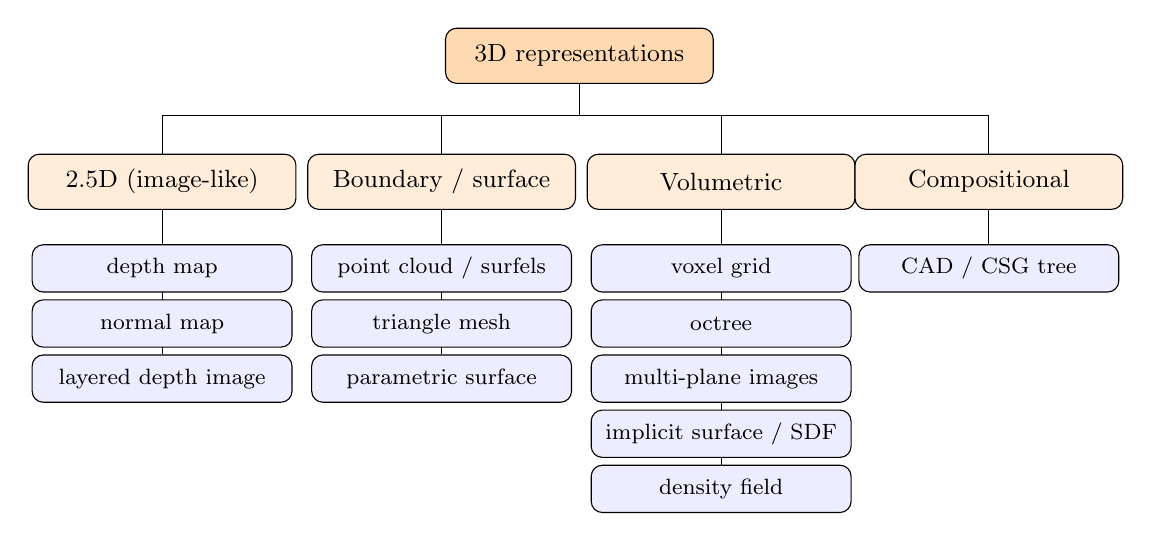
\begin{tikzpicture}[font=\small,
  lvl/.style={draw,rounded corners,fill=orange!15,minimum height=7mm,minimum width=3.4cm,align=center},
  ch/.style={draw,rounded corners,fill=blue!7,minimum height=6mm,minimum width=3.3cm,align=center,font=\footnotesize}]
\node[lvl,fill=orange!30] (root) at (0,0) {3D representations};
\node[lvl] (h) at (-5.3,-1.6) {2.5D (image-like)};
\node[lvl] (b) at (-1.75,-1.6) {Boundary / surface};
\node[lvl] (v) at (1.8,-1.6) {Volumetric};
\node[lvl] (c) at (5.2,-1.6) {Compositional};
\foreach \p in {h,b,v,c}{\draw (root.south) -- ++(0,-0.4) -| (\p.north);}
\node[ch] (h1) at (-5.3,-2.7) {depth map};
\node[ch] (h2) at (-5.3,-3.4) {normal map};
\node[ch] (h3) at (-5.3,-4.1) {layered depth image};
\node[ch] (b1) at (-1.75,-2.7) {point cloud / surfels};
\node[ch] (b2) at (-1.75,-3.4) {triangle mesh};
\node[ch] (b3) at (-1.75,-4.1) {parametric surface};
\node[ch] (v1) at (1.8,-2.7) {voxel grid};
\node[ch] (v2) at (1.8,-3.4) {octree};
\node[ch] (v3) at (1.8,-4.1) {multi-plane images};
\node[ch] (v4) at (1.8,-4.8) {implicit surface / SDF};
\node[ch] (v5) at (1.8,-5.5) {density field};
\node[ch] (c1) at (5.2,-2.7) {CAD / CSG tree};
\begin{scope}[on background layer]
\draw (h.south) -- (h3.north);
\draw (b.south) -- (b3.north);
\draw (v.south) -- (v5.north);
\draw (c.south) -- (c1.north);
\end{scope}
\end{tikzpicture}
\caption{A map of the representations met in the lecture (our grouping, following slides 43 and 63: points, meshes and parametric surfaces are \emph{boundary} representations; voxels and implicit fields are \emph{volumetric}).}
\end{figure}

% =====================================================================
\section{Notation \slides{slide 5}}
% =====================================================================

\begin{definition}[Notation]
A point in 3D space is written in inhomogeneous coordinates as
\[
\vx=\begin{pmatrix}x\\y\\z\end{pmatrix}\in\R^3 .
\]
A point on the image plane carries the subscript $s$: $\vx_s\in\R^2$. Discrete maps are \emph{indexed} rather than evaluated, and brackets denote indexing:
\[
D[\vx_s]\in\R^+ \quad(\text{depth}),\qquad N[\vx_s]\in\Sph^2 \quad(\text{unit normal}),\qquad V[i,j,k]\in[0,1]\quad(\text{occupancy}).
\]
\end{definition}

\begin{remark}
The subscript denotes the \emph{coordinate frame}, not the dimension of the space. Both $\vx$ and $\vx_s$ denote points.
\end{remark}

\begin{intuition}
Parentheses mean ``compute'' ($f(\vx)$ runs a formula or a network); brackets mean ``look up'' ($D[\vx_s]$ reads a pixel). The letter $s$ is a hint that $\vx_s$ lives on the \emph{s}creen; it is a name tag, not an exponent.
\end{intuition}

% =====================================================================
\section{Manifolds \slides{slide 6}}
% =====================================================================

\begin{definition}[Manifold]
An $n$-dimensional \emph{manifold} is a topological space that locally resembles Euclidean space: every point has a neighborhood homeomorphic to an open subset of $\R^n$; $n$ is its dimension.
\end{definition}

Lines and circles are $1$-manifolds. Two-dimensional manifolds are called \emph{surfaces}: the plane, the sphere, the torus. Each coloured piece of the shape on the slide is a \emph{chart}: it flattens a part of the shape onto $\R^n$.

\begin{figure}[ht]
\centering
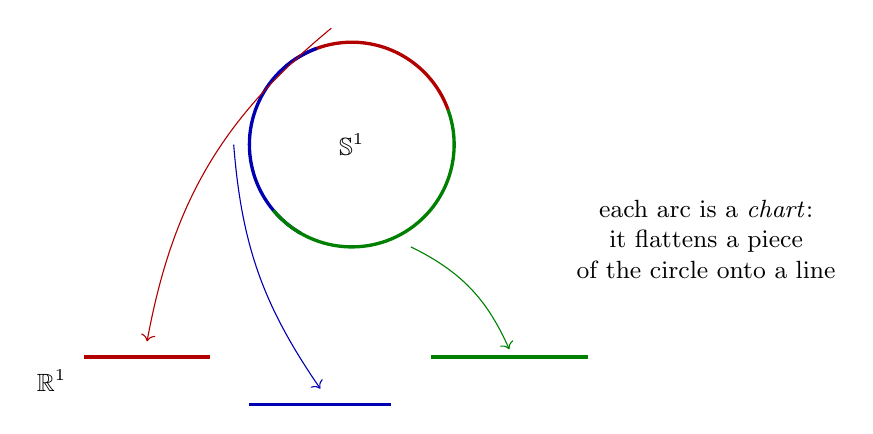
\begin{tikzpicture}[font=\small,scale=1]
\draw[gray!50] (0,0) circle (1.3);
\draw[very thick,red!70!black] (0,0)++(20:1.3) arc (20:130:1.3);
\draw[very thick,blue!70!black] (0,0)++(110:1.3) arc (110:240:1.3);
\draw[very thick,green!50!black] (0,0)++(220:1.3) arc (220:380:1.3);
\node at (0,0) {$\Sph^1$};
\begin{scope}[yshift=-3.3cm]
\draw[very thick,red!70!black] (-3.4,0.6) -- (-1.8,0.6);
\draw[very thick,blue!70!black] (-1.3,0) -- (0.5,0);
\draw[very thick,green!50!black] (1.0,0.6) -- (3.0,0.6);
\node[left] at (-3.5,0.3) {$\R^1$};
\end{scope}
\draw[->,red!70!black] (100:1.5) to[bend right=20] (-2.6,-2.5);
\draw[->,blue!70!black] (180:1.5) to[bend right=15] (-0.4,-3.1);
\draw[->,green!50!black] (300:1.5) to[bend left=20] (2.0,-2.6);
\node[align=center] at (4.5,-1.2) {each arc is a \emph{chart}:\\it flattens a piece\\of the circle onto a line};
\end{tikzpicture}
\caption{The circle is a $1$-manifold. Three overlapping charts, each a homeomorphism from an arc to an interval of $\R$, cover it. (Slide 6 shows the same idea for a circle and a sphere.)}
\end{figure}

\begin{intuition}
An ant walking on a sphere sees a flat plane around itself: that local flatness is what ``manifold'' means. The sphere as a whole is \emph{not} a plane, which is why one needs several overlapping charts (an atlas) to describe it, exactly as one needs several flat maps to cover the Earth without cutting it.
\end{intuition}

% =====================================================================
\section{Defining a Surface \slides{slide 7}}
% =====================================================================

\begin{definition}[Parametric and implicit forms]
A surface can be specified in two ways.
\begin{itemize}[nosep]
\item \textbf{Parametric form:} a function maps a 2D domain into space,
$f(\vu)=\vx\in\R^3,\ \vu\in\M$.
\item \textbf{Implicit form:} the surface is the zero level set of a scalar field, $\Surf=\{\vx\mid f(\vx)=0\}$.
\end{itemize}
In the parametric form the domain point $\vu$ is \emph{not} a point in space: it belongs to a 2D manifold $\M$, for instance the sphere $\Sph^2$.
\end{definition}

\begin{remark}
The symbol $f$ denotes both functions; the argument decides which is meant: $f(\vu)$ returns a surface point, $f(\vx)$ returns a scalar.
\end{remark}

\begin{intuition}
Parametric = ``a recipe that \emph{produces} points'' (feed in a domain point, get a 3D point out). Implicit = ``a rule that \emph{judges} points'' (feed in a 3D point, get a number whose sign says on which side of the surface it lies). Slide 48 will turn this into the mantra \emph{parametric generates, implicit tests}.
\end{intuition}

% =====================================================================
\section{Meanwhile in 3D-land\dots\ \slides{slides 8--9}}
% =====================================================================

``But what is the \emph{best} representation?'' The slide's answer: \emph{it depends}, on the task: acquisition vs editing vs animation vs prediction vs processing vs optimization, and more.

The goals of the lecture (slide 9):
\begin{itemize}[nosep]
\item understand representations \emph{computationally} (what do they look like in code?);
\item understand their limitations and benefits;
\item understand conversions across representations.
\end{itemize}

\begin{intuition}
There is no free lunch: a representation that makes one operation trivial tends to make another one painful. Reading each representation below, ask three questions: how do I \emph{store} it, what is \emph{easy} to do with it, what is \emph{hard}?
The lecture proceeds from representations tied to sensors (depth maps, point clouds), through surfaces (meshes, parametric surfaces), to volumes (voxels, implicit fields, density fields).
\end{intuition}

% =====================================================================
\section{Depth Maps \slides{slides 10--14}}
% =====================================================================

\subsection{Depth maps \slides{slides 10--12}}
Depth is a \emph{common modality across sensors} (structured-light and time-of-flight cameras such as the Kinect and industrial cameras shown on slide 10); depth is treated in detail in Lectures 04--05.

\begin{definition}[Depth map]
A depth map is an image $D[\vx_s]\in\R^+$ that records how far the scene point seen by each pixel $\vx_s$ is from the camera.
\end{definition}

Because it is just an image, \emph{standard image-processing tools can be used} on it (slide 12): filtering, resizing, convolutional networks.

\subsection{Depth Maps and Normal Maps \slides{slide 13}}
The same idea extends to other surface properties, e.g.\ surface normals:
\begin{definition}[Normal map]
$N[\vx_s]\in\Sph^2$ stores, for each pixel, the unit normal of the visible surface.
\end{definition}

\begin{figure}[H]
\centering
\includegraphics[width=0.75\textwidth]{tex/EAI02/depth_normal.png}
\caption{Depth and normal maps of a scene. The depth map is a grayscale image where brightness encodes distance; the normal map is a color image where RGB encodes the XYZ components of the unit normal.}
\end{figure}


\subsection{Depth Maps --- Representing the Visible \slides{slide 14}}
\begin{remark}
A depth map does not capture the \emph{full} 3D structure: it is a \emph{2.5D} representation, i.e.\ properties associated with image pixels. The slide asks: can we develop more \emph{complete} 3D representations?
\end{remark}

\begin{figure}[ht]
\centering
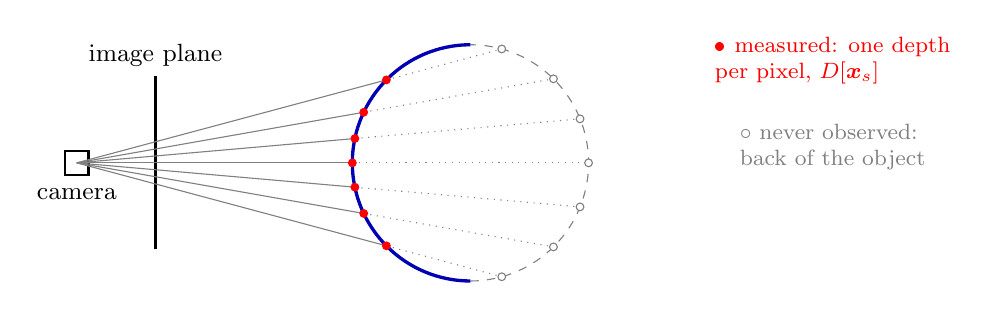
\begin{tikzpicture}[font=\small]
\draw[thick] (-0.15,-0.15) rectangle (0.15,0.15); \node[below] at (0,-0.2) {camera};
\draw[thick] (1,-1.1) -- (1,1.1); \node[above] at (1,1.1) {image plane};
\draw[dashed,gray] (5,0)++(-90:1.5) arc (-90:90:1.5);
\draw[very thick,blue!70!black] (5,0)++(90:1.5) arc (90:270:1.5);
\foreach \a in {-15,-10,-5,0,5,10,15}{
  \pgfmathsetmacro{\t}{5*cos(\a)-sqrt((5*cos(\a))^2-22.75)}
  \pgfmathsetmacro{\tb}{5*cos(\a)+sqrt((5*cos(\a))^2-22.75)}
  \draw[gray] (0,0) -- (\a:\t);
  \draw[dotted,gray] (\a:\t) -- (\a:\tb);
  \fill[red] (\a:\t) circle (1.6pt);
  \draw[gray,fill=white] (\a:\tb) circle (1.4pt);
}
\node[red,align=left,font=\footnotesize] at (9.6,1.3) {\textbullet\ measured: one depth\\per pixel, $D[\vx_s]$};
\node[gray,align=left,font=\footnotesize] at (9.6,0.2) {$\circ$ never observed:\\back of the object};
\end{tikzpicture}
\caption{Side view of a depth camera. Each pixel ray returns the \emph{first} surface hit (red); the far side of the object (dashed) and anything hidden behind the visible surface is absent from $D$.}
\end{figure}

\begin{intuition}
A depth map is like a relief map seen from one viewpoint: it tells the distance to whatever is \emph{in front}, and nothing about what is behind it. Two things follow. First, cheap and fast: it is an ordinary image. Second, incomplete: to model a whole object you need several views or a representation that lives in 3D itself, which motivates point clouds next.
\end{intuition}

% =====================================================================
\section{Point Clouds \slides{slides 15--21}}
% =====================================================================

\subsection{Point Clouds \slides{slides 15--18}}
\begin{figure}[H]
\centering
\includegraphics[width=0.75\textwidth]{tex/EAI02/pointcloud.png}
\caption{Some point clouds of scenes. Each point is a 3D position, and can be drawn as a small sphere.}
\end{figure}

Point clouds are often acquired in an image-like manner from sensors (LiDAR, depth cameras) but it can be useful to \emph{forget} this: point clouds from multiple views can be merged into a single point cloud, which helps unify approaches independently of the sensing modality.

\begin{definition}[Point cloud]
A point cloud is an \emph{unordered set} of points $\{\vx_1,\vx_2,\dots,\vx_N\}\subset\R^3$, usually stored as an $N\times 3$ array. Reordering the rows by any permutation $\sigma$ gives $\{\vx_{\sigma(1)},\dots,\vx_{\sigma(N)}\}$, the \emph{same} point cloud.
\end{definition}

Unlike an image, the row order carries no meaning, so processing or generation methods must be \emph{permutation invariant}; a fully connected layer applied to the flattened array does not work.

\begin{example}[Why a fully connected layer fails]
Let $X=\{\vx_1=(1,0,0),\,\vx_2=(0,1,0)\}$. Flattened, the two orderings give $(1,0,0,0,1,0)$ and $(0,1,0,1,0,0)$, two different vectors, so a generic linear layer returns two different outputs for one geometric object. A \emph{symmetric} operation such as taking the per-coordinate maximum over the points returns $(1,1,0)$ in both orders.
\end{example}

\begin{intuition}
Think of a bag of marbles: shaking it does not change what it contains. An operator must treat the input as a bag, not as a list. Symmetric functions (sum, mean, max over points) have this property, and network designs for point clouds are built from them.
\end{intuition}

\subsection{Oriented Point Clouds \slides{slide 19}}
\begin{definition}[Oriented point cloud, surfel]
An oriented point cloud stores a normal with each point: $\{(\vx_1,\vn_1),\dots,(\vx_N,\vn_N)\}$. Points can then be treated as small flat disks rather than tiny spheres, which helps rendering under lighting. When a radius is also stored the primitives are called \emph{surfels}.
\end{definition}

\begin{figure}[ht]
\centering
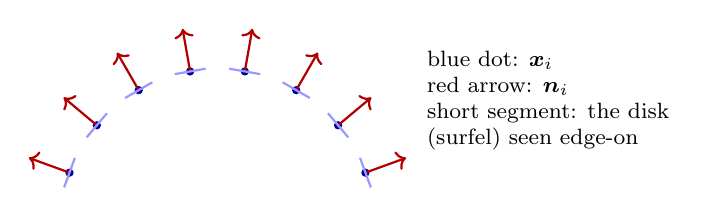
\begin{tikzpicture}[font=\small]
\foreach \a in {20,40,...,160}{
  \fill[blue!60!black] (\a:2) circle (1.5pt);
  \draw[->,red!70!black,thick] (\a:2) -- (\a:2.55);
  \draw[thick,blue!40] ($(\a:2)+(\a+90:0.2)$) -- ($(\a:2)+(\a-90:0.2)$);
}
\node[align=left,font=\footnotesize] at (4.2,1.6) {blue dot: $\vx_i$\\red arrow: $\vn_i$\\short segment: the disk\\(surfel) seen edge-on};
\end{tikzpicture}
\caption{An oriented point cloud sampled from a curve (2D cross-section): each sample carries a position and a normal, and can be drawn as a small disk perpendicular to the normal.}
\end{figure}

\begin{figure}[H]
\centering
\includegraphics[width=0.75\textwidth]{tex/EAI02/surfels.png}
\caption{A surfel-based reconstruction of a dinosaur. Each surfel is a small disk with a position, a normal and a radius.}
\end{figure}


\begin{intuition}
A bare point has no facing direction, so lighting is ambiguous. Attaching a normal turns each point into a tiny mirror; adding a radius makes the mirror cover a patch of surface, so neighbours overlap and the gaps between samples close up.
\end{intuition}

\subsection{No explicit connectivity \slides{slides 20--21}}
A point cloud has no explicit \emph{connectivity} information. Two point sets that look nearly identical may come from a closed circle and from a circle with a small gap. One can always sample more points to resolve the gap, but this is super inefficient; it is more efficient to add \emph{edges}, because connectivity does not scale like density (which grows with an area).

\begin{figure}[ht]
\centering
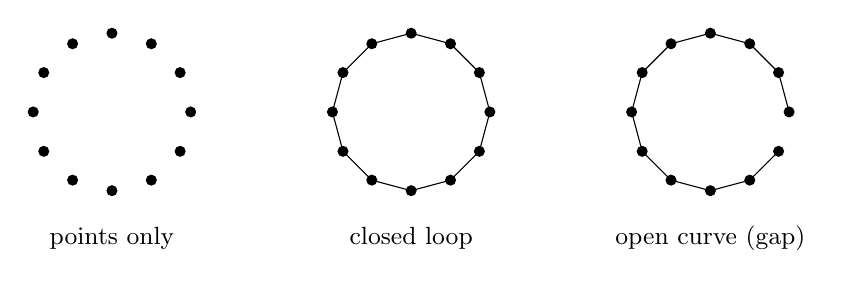
\begin{tikzpicture}[font=\small]
\foreach \i in {0,...,11}{\fill (30*\i:1) circle (2pt);}
\node at (0,-1.6) {points only};
\begin{scope}[xshift=3.8cm]
\foreach \i/\j in {0/1,1/2,2/3,3/4,4/5,5/6,6/7,7/8,8/9,9/10,10/11,11/0}{\draw (30*\i:1) -- (30*\j:1);}
\foreach \i in {0,...,11}{\fill (30*\i:1) circle (2pt);}
\node at (0,-1.6) {closed loop};
\end{scope}
\begin{scope}[xshift=7.6cm]
\foreach \i/\j in {0/1,1/2,2/3,3/4,4/5,5/6,6/7,7/8,8/9,9/10,10/11}{\draw (30*\i:1) -- (30*\j:1);}
\foreach \i in {0,...,11}{\fill (30*\i:1) circle (2pt);}
\node at (0,-1.6) {open curve (gap)};
\end{scope}
\end{tikzpicture}
\caption{The same 12 points support two different shapes: only the edges (connectivity) tell them apart.}
\end{figure}

\begin{example}[Density vs.\ connectivity]
To sample a unit sphere with spacing $h$ one needs roughly $4\pi/h^2$ points: about $1257$ for $h=0.1$ but about $5027$ for $h=0.05$. Halving the spacing multiplies the number of points by $4$, while adding one edge costs one pair of integers.
\end{example}

\begin{intuition}
Density is a \emph{2D} bill (points per unit area), connectivity is a \emph{1D} one (a few edges along features). To say ``these two neighbouring points belong to the same continuous piece'' it is far cheaper to draw a line than to fill the gap with hundreds of extra samples. This is exactly what meshes do.
\end{intuition}

% =====================================================================
\section{Meshes \slides{slides 22--34}}
% =====================================================================

\subsection{Meshes: vertices and faces \slides{slides 22--25}}
Meshes are \emph{piecewise linear approximations} of the underlying surface; more elements allow a better approximation (slide 22 shows a torus with increasing resolution).

\begin{figure}[H]
\centering
\includegraphics[width=0.75\textwidth]{tex/EAI02/mesh_torus.png}
\caption{A torus approximated by a mesh of increasing resolution and the difference between a mesh and a pointcloud of a rabbit. The mesh is a
 piecewise linear approximation of the underlying surface.}
\end{figure}
\begin{definition}[Mesh]
A mesh is a pair $(V,F)$: $V$ is an $N\times 3$ array of vertex positions (the \emph{geometry}) and $F$ is a list of $M$ faces (the \emph{topology}), each face being a list of indices of the vertices that make it up. Consecutive indices in a face are joined by an edge, so \emph{ordering matters} in face indices.
\end{definition}

\begin{figure}[ht]
\centering
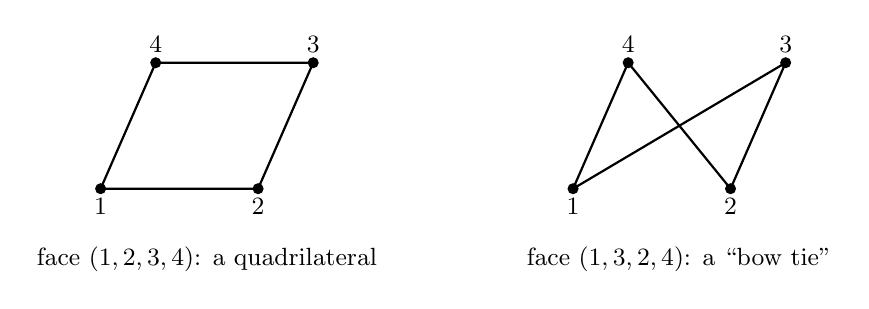
\begin{tikzpicture}[font=\small]
\begin{scope}
\draw[thick] (0,0)--(2,0)--(2.7,1.6)--(0.7,1.6)--cycle;
\foreach \p/\l/\pos in {(0,0)/1/below,(2,0)/2/below,(2.7,1.6)/3/above,(0.7,1.6)/4/above}{\fill \p circle (2pt); \node[\pos] at \p {\l};}
\node at (1.35,-0.9) {face $(1,2,3,4)$: a quadrilateral};
\end{scope}
\begin{scope}[xshift=6cm]
\draw[thick] (0,0)--(2.7,1.6)--(2,0)--(0.7,1.6)--cycle;
\foreach \p/\l/\pos in {(0,0)/1/below,(2,0)/2/below,(2.7,1.6)/3/above,(0.7,1.6)/4/above}{\fill \p circle (2pt); \node[\pos] at \p {\l};}
\node at (1.35,-0.9) {face $(1,3,2,4)$: a ``bow tie''};
\end{scope}
\end{tikzpicture}
\caption{Same four vertices, two index orders, two different shapes: consecutive indices are connected by an edge.}
\end{figure}

Arbitrary polygons can also be \emph{non-planar} (four points in 3D need not lie in a plane), so one restricts to triangles: three points not on a line always define a plane.

\begin{figure}[ht]
\centering
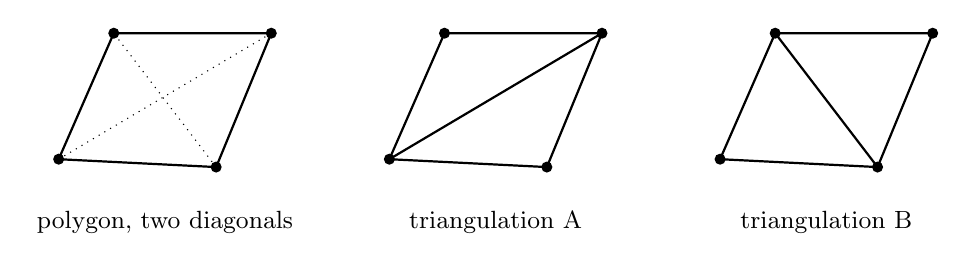
\begin{tikzpicture}[font=\small]
\foreach \dx/\kind in {0/0,4.2/1,8.4/2}{
 \begin{scope}[xshift=\dx cm]
 \draw[thick] (0,0)--(2,-0.1)--(2.7,1.6)--(0.7,1.6)--cycle;
 \ifnum\kind=0 \draw[dotted] (0,0)--(2.7,1.6); \draw[dotted] (2,-0.1)--(0.7,1.6); \fi
 \ifnum\kind=1 \draw[thick] (0,0)--(2.7,1.6); \fi
 \ifnum\kind=2 \draw[thick] (2,-0.1)--(0.7,1.6); \fi
 \foreach \p in {(0,0),(2,-0.1),(2.7,1.6),(0.7,1.6)}{\fill \p circle (2pt);}
 \end{scope}
}
\node at (1.35,-0.8) {polygon, two diagonals};
\node at (5.55,-0.8) {triangulation A};
\node at (9.75,-0.8) {triangulation B};
\end{tikzpicture}
\caption{A quad can be split into triangles in two ways. If the four points are not coplanar, A and B are two genuinely different surfaces, while each triangle on its own is always flat.}
\end{figure}

\subsection{Triangular Meshes \slides{slides 26--31}}
\begin{definition}[Triangular mesh]
A triangular mesh is a mesh whose faces are all triangles: $V\in\R^{N\times 3}$ and $F\in\{0,\dots,N-1\}^{M\times 3}$, each row of $F$ listing the indices of the \emph{three} vertices of a face.
\end{definition}

\begin{example}[A tetrahedron in code]
\begin{lstlisting}
V = np.array([[0,0,0],[1,0,0],[0,1,0],[0,0,1]], dtype=float)   # 4 x 3
F = np.array([[0,2,1],[0,1,3],[0,3,2],[1,2,3]])                # 4 x 3, ints
\end{lstlisting}
Here $N=4$ vertices, $M=4$ faces and $E=6$ edges.
\end{example}

\paragraph{A sanity check on sizes.}
\begin{proposition}[Face count of a closed genus-0 triangle mesh]\label{prop:euler}
Let a closed, sphere-like (genus~0) triangular mesh have $V$ vertices, $E$ edges and $F$ faces. Every face has $3$ edges and every edge is shared by $2$ faces, so $E=3F/2$. With Euler's formula $V-E+F=2$ this gives
\[
F=2V-4 .
\]
\end{proposition}
\begin{proof}
Substitute $E=3F/2$ into $V-E+F=2$: $V-\tfrac32F+F=2$, i.e.\ $V-\tfrac12F=2$, hence $F=2V-4$.
\end{proof}

\begin{intuition}
You get about \emph{twice as many triangles as vertices}. Checks: tetrahedron $V=4\Rightarrow F=4$ \checkmark; octahedron $V=6\Rightarrow F=8$ \checkmark; a scan with $V=10{,}000$ vertices has $F=19{,}996$ faces and $E=3F/2=29{,}994$ edges. Useful to guess memory footprints or to spot a broken mesh.
\end{intuition}

\paragraph{Orientation.} For a triangle, \emph{any order gives the same triangle}, but the order determines which side is ``front''. The normal is $\vn=(\vb-\va)\times(\vc-\va)$.

\begin{proposition}[Orientation and index order]\label{prop:orient}
A cyclic shift $(a,b,c)\to(b,c,a)$ leaves $\vn$ unchanged; swapping two indices, e.g.\ $(a,b,c)\to(c,b,a)$, flips its sign.
\end{proposition}
\begin{proof}
Expanding, $(\vb-\va)\times(\vc-\va)=\vb\times\vc-\vb\times\va-\va\times\vc+\va\times\va=\va\times\vb+\vb\times\vc+\vc\times\va$. This expression is unchanged by cyclic relabelling $\va\to\vb\to\vc\to\va$ and changes sign under the swap of any two symbols, since $\times$ is antisymmetric.
\end{proof}

\begin{figure}[ht]
\centering
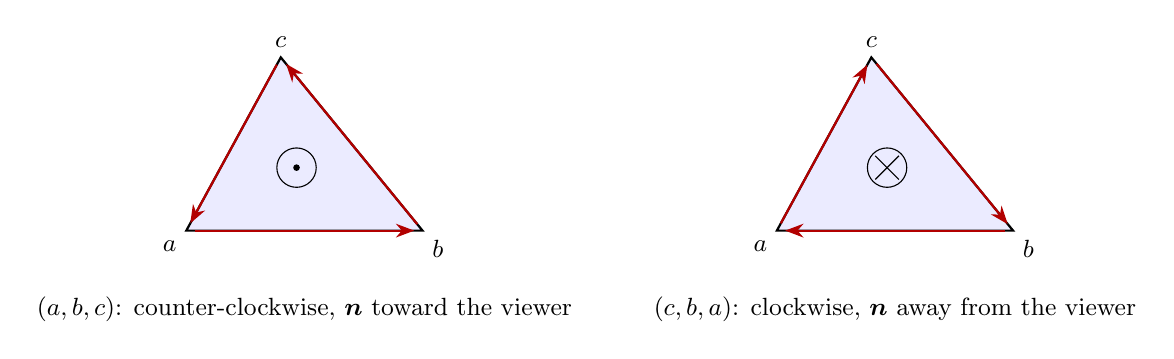
\begin{tikzpicture}[font=\small,>=Stealth]
\begin{scope}
\coordinate (a) at (0,0); \coordinate (b) at (3,0); \coordinate (c) at (1.2,2.2);
\draw[thick,fill=blue!8] (a)--(b)--(c)--cycle;
\draw[->,thick,red!70!black,shorten >=3pt,shorten <=3pt] (a)--(b);
\draw[->,thick,red!70!black,shorten >=3pt,shorten <=3pt] (b)--(c);
\draw[->,thick,red!70!black,shorten >=3pt,shorten <=3pt] (c)--(a);
\node[below left] at (a) {$a$}; \node[below right] at (b) {$b$}; \node[above] at (c) {$c$};
\node[draw,circle,inner sep=0pt,minimum size=5mm] at (1.4,0.8) {}; \fill (1.4,0.8) circle (1.2pt);
\node at (1.5,-1) {$(a,b,c)$: counter-clockwise, $\vn$ toward the viewer};
\end{scope}
\begin{scope}[xshift=7.5cm]
\coordinate (a) at (0,0); \coordinate (b) at (3,0); \coordinate (c) at (1.2,2.2);
\draw[thick,fill=blue!8] (a)--(b)--(c)--cycle;
\draw[->,thick,red!70!black,shorten >=3pt,shorten <=3pt] (c)--(b);
\draw[->,thick,red!70!black,shorten >=3pt,shorten <=3pt] (b)--(a);
\draw[->,thick,red!70!black,shorten >=3pt,shorten <=3pt] (a)--(c);
\node[below left] at (a) {$a$}; \node[below right] at (b) {$b$}; \node[above] at (c) {$c$};
\node[draw,circle,inner sep=0pt,minimum size=5mm] at (1.4,0.8) {}; 
\draw (1.25,0.65)--(1.55,0.95); \draw (1.25,0.95)--(1.55,0.65);
\node at (1.5,-1) {$(c,b,a)$: clockwise, $\vn$ away from the viewer};
\end{scope}
\end{tikzpicture}
\caption{Index order defines the winding direction and hence the side the normal points to. Swapping two indices reverses it.}
\end{figure}

\begin{example}[Checking the tetrahedron]
For face $(0,2,1)$ of the example above, $\va=(0,0,0)$, $\vb=(0,1,0)$, $\vc=(1,0,0)$: $\vn=(0,1,0)\times(1,0,0)=(0,0,-1)$, pointing down, i.e.\ \emph{outward} for the face lying in $z=0$ (the tetrahedron sits above it). Face $(1,2,3)$ gives $(-1,1,0)\times(-1,0,1)=(1,1,1)$, also outward. All four faces are consistently oriented.
\end{example}

\begin{intuition}
The ``classic bug'': if some faces are listed clockwise and others counter-clockwise, the renderer treats some triangles as back-facing and they render black or vanish. Rule of thumb: use one winding convention for the whole mesh and check with $\vn$ pointing away from the interior.
\end{intuition}

\paragraph{Manifold problems.}
Even with triangles one can still get \emph{non-manifold} meshes. The slides identify two cases: an edge shared by more than two faces (so restrict each edge to at most two faces; one can often get away without enforcing this) and a \emph{disconnected surface around a vertex}, which is critical for mesh-processing applications and less so for rendering.

\begin{figure}[ht]
\centering
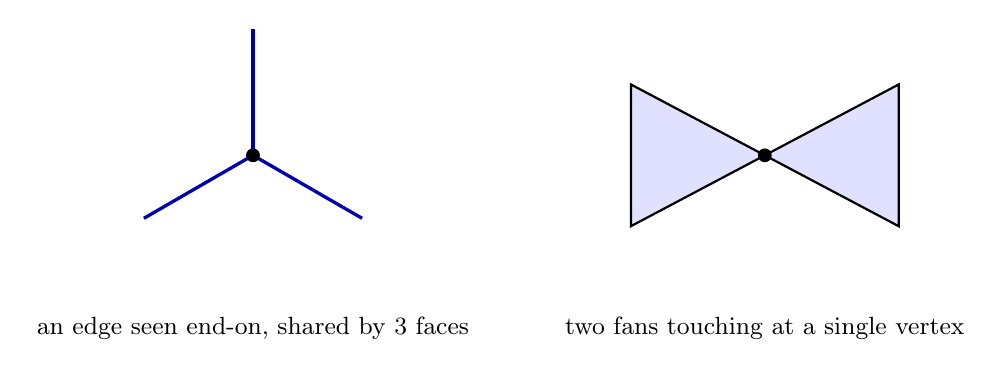
\begin{tikzpicture}[font=\small]
\begin{scope}
\foreach \a in {90,210,330}{\draw[very thick,blue!70!black] (0,0) -- (\a:1.6);}
\fill (0,0) circle (2.5pt);
\node at (0,-2.2) {an edge seen end-on, shared by 3 faces};
\end{scope}
\begin{scope}[xshift=6.5cm]
\draw[thick,fill=blue!12] (0,0) -- (-1.7,0.9) -- (-1.7,-0.9) -- cycle;
\draw[thick,fill=blue!12] (0,0) -- (1.7,0.9) -- (1.7,-0.9) -- cycle;
\fill (0,0) circle (2.5pt);
\node at (0,-2.2) {two fans touching at a single vertex};
\end{scope}
\end{tikzpicture}
\caption{Two kinds of non-manifold configuration.}
\end{figure}

\paragraph{Ray--triangle intersection and texturing.}
\begin{proposition}[Barycentric form and the ray--triangle solve]\label{prop:ray}
Any point of the triangle with vertices $\va,\vb,\vc$ is $\alpha\va+\beta\vb+\gamma\vc$ with $\alpha+\beta+\gamma=1$ and all three weights $\ge 0$. Setting this equal to the ray $\vo+t\vd$ gives $3$ linear equations in the $3$ unknowns $(t,\beta,\gamma)$, i.e.\ a $3\times 3$ solve per triangle:
\[
\beta(\vb-\va)+\gamma(\vc-\va)-t\,\vd=\vo-\va ,\qquad \alpha=1-\beta-\gamma .
\]
The ray hits the triangle iff $\beta\ge0$, $\gamma\ge0$, $\beta+\gamma\le 1$ (and $t>0$).
\end{proposition}
\begin{proof}
Substitute $\alpha=1-\beta-\gamma$ in $\alpha\va+\beta\vb+\gamma\vc=\vo+t\vd$ and collect terms.
\end{proof}

\begin{example}
Triangle $\va=(0,0,0)$, $\vb=(1,0,0)$, $\vc=(0,1,0)$; ray $\vo=(0.25,0.25,1)$, $\vd=(0,0,-1)$. The system reads $\beta(1,0,0)+\gamma(0,1,0)-t(0,0,-1)=(0.25,0.25,1)$, so $\beta=\gamma=0.25$, $t=1$, $\alpha=0.5$. All weights are $\ge0$: hit at $\vo+\vd=(0.25,0.25,0)$.
\end{example}

Texturing is easy: each vertex also stores a coordinate into a 2D image, and inside a triangle the same weights interpolate those coordinates.

\begin{figure}[ht]
\centering
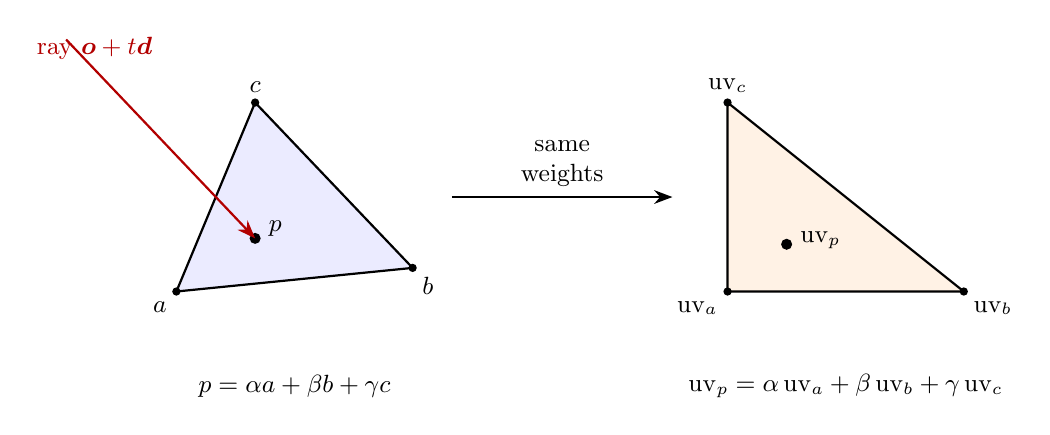
\begin{tikzpicture}[font=\small,>=Stealth]
\coordinate (a) at (0,0); \coordinate (b) at (3,0.3); \coordinate (c) at (1,2.4);
\coordinate (p) at (1,0.675);
\draw[thick,fill=blue!8] (a)--(b)--(c)--cycle;
\fill (p) circle (2pt);
\foreach \v/\l/\pos in {a/a/below left,b/b/below right,c/c/above}{\fill (\v) circle (1.5pt); \node[\pos] at (\v) {$\l$};}
\node[right] at (1.05,0.8) {$p$};
\draw[->,thick,red!70!black] (-1.4,3.2) -- (p) node[pos=0.15,above] {ray $\vo+t\vd$};
\node[align=center] at (1.5,-1.2) {$p=\alpha a+\beta b+\gamma c$};
\begin{scope}[xshift=7cm]
\coordinate (a2) at (0,0); \coordinate (b2) at (3,0); \coordinate (c2) at (0,2.4);
\coordinate (p2) at (0.75,0.6);
\draw[thick,fill=orange!10] (a2)--(b2)--(c2)--cycle;
\fill (p2) circle (2pt);
\foreach \v/\l/\pos in {a2/{a}/below left,b2/{b}/below right,c2/{c}/above}{\fill (\v) circle (1.5pt); \node[\pos] at (\v) {$\mathrm{uv}_\l$};}
\node[right] at (0.8,0.65) {$\mathrm{uv}_p$};
\node[align=center] at (1.5,-1.2) {$\mathrm{uv}_p=\alpha\,\mathrm{uv}_a+\beta\,\mathrm{uv}_b+\gamma\,\mathrm{uv}_c$};
\end{scope}
\draw[->,thick] (3.5,1.2) -- (6.3,1.2) node[midway,above,align=center] {same\\weights};
\end{tikzpicture}
\caption{Left: the hit point in barycentric coordinates $(\alpha,\beta,\gamma)=(0.5,0.25,0.25)$. Right: the same weights interpolate the 2D texture coordinates stored at the vertices.}
\end{figure}

\begin{intuition}
Barycentric weights are ``how much of each corner'' a point is made of; a point near $a$ has $\alpha$ close to $1$. Intersecting a ray with a triangle is therefore a tiny linear-algebra problem, which is why GPUs can do billions of them, and the \emph{same} weights carry any per-vertex quantity (texture coordinates, colours, normals) to the interior.
\end{intuition}

\subsection{Triangular Meshes --- Geometry vs Connectivity \slides{slides 32--34}}
The two arrays of a mesh behave very differently:
$V$ is \texttt{float}, differentiable, and gradient descent (GD) is happy; $F$ is \texttt{int}, discrete, and GD is not happy. Modifying vertex positions can edit the shape; other changes are non-trivial (i.e.\ changing $F$).

\begin{figure}[H]
\centering
\includegraphics[width=0.75\textwidth]{tex/EAI02/geometry_connectivity.png}
\caption{Editing the geometry $V$ is easy, editing the connectivity $F$ is hard.}
\end{figure}

\begin{figure}[ht]
\centering
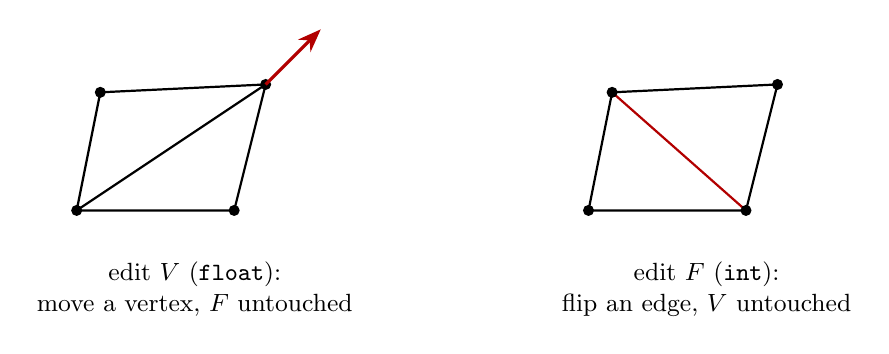
\begin{tikzpicture}[font=\small,>=Stealth]
\begin{scope}
\draw[thick] (0,0)--(2,0)--(2.4,1.6)--(0.3,1.5)--cycle; \draw[thick] (0,0)--(2.4,1.6);
\foreach \p in {(0,0),(2,0),(2.4,1.6),(0.3,1.5)}{\fill \p circle (2pt);}
\draw[->,red!70!black,very thick] (2.4,1.6) -- (3.1,2.3);
\node[align=center] at (1.5,-1) {edit $V$ (\texttt{float}):\\move a vertex, $F$ untouched};
\end{scope}
\begin{scope}[xshift=6.5cm]
\draw[thick] (0,0)--(2,0)--(2.4,1.6)--(0.3,1.5)--cycle; \draw[thick,red!70!black] (2,0)--(0.3,1.5);
\foreach \p in {(0,0),(2,0),(2.4,1.6),(0.3,1.5)}{\fill \p circle (2pt);}
\node[align=center] at (1.5,-1) {edit $F$ (\texttt{int}):\\flip an edge, $V$ untouched};
\end{scope}
\end{tikzpicture}
\caption{Geometry edits are small continuous changes of real numbers; connectivity edits are combinatorial jumps.}
\end{figure}

\subsubsection*{Same counts, different meshes \slides{slide 33}}
Going from one mesh to another is non-trivial even when both have $6$ vertices and $8$ faces (the octahedron is one such mesh). It is even more challenging if the topology changes, e.g.\ torus to sphere. In general, designing methods that can predict \emph{arbitrary} connectivity is challenging (e.g.\ image to mesh).
\begin{figure}[H]
\centering
\includegraphics[width=0.75\textwidth]{tex/EAI02/mesh_edit.png}
\caption{Two meshes with the same number of vertices and faces, but different connectivity.}
\end{figure}
\subsubsection*{Continuous deformation \slides{slide 34}}
The first change (same counts, different connectivity) is possible under continuous deformation of the shape; the torus-to-sphere change is impossible under continuous deformation (a hole cannot be closed without tearing). Yet \emph{both} edits require similar operations for meshes: a new $F$ and an updated $V$. The slide asks: is there an alternate representation where the former (the continuous one) is easier?

\begin{intuition}
A mesh mixes a smooth part ($V$) with a rigid combinatorial part ($F$). Even a tiny, continuous change of the shape may demand a jump in $F$, and a network cannot easily output ``an integer array of unknown length''. The question hanging in the air motivates representations where shape changes are always changes of continuous numbers: parametric and, above all, implicit ones.
\end{intuition}

% =====================================================================
\section{Parametric Surfaces \slides{slides 35--41}}
% =====================================================================

\subsection{Parametric surfaces in 2D \slides{slide 35}}
The domain is a circle $\Sph^1$; think of it as an angle $\theta$. A function $f(\vu)=\vx\in\R^2,\ \vu\in\Sph^1$ sends each angle to a point of a curve: $f_1$ to a pentagon, $f_2$ to a square.

\begin{figure}[ht]
\centering
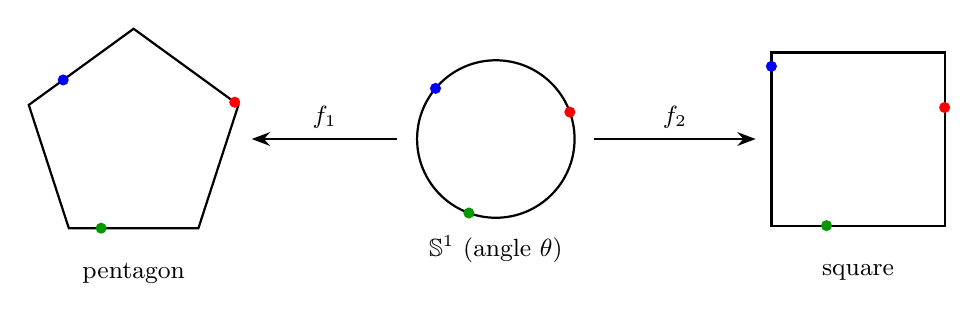
\begin{tikzpicture}[font=\small,>=Stealth]
\draw[thick] (0,0) circle (1);
\foreach \th/\col in {20/red,140/blue,250/green!60!black}{\fill[\col] (\th:1) circle (2pt);}
\node at (0,-1.4) {$\Sph^1$ (angle $\theta$)};
\begin{scope}[xshift=-4.6cm]
\draw[thick] (90:1.4)--(162:1.4)--(234:1.4)--(306:1.4)--(18:1.4)--cycle;
\foreach \th/\col in {20/red,140/blue,250/green!60!black}{
  \pgfmathsetmacro{\ph}{72*round((\th-54)/72)+54}
  \pgfmathsetmacro{\rr}{1.4*cos(36)/cos(\th-\ph)}
  \fill[\col] (\th:\rr) circle (2pt);}
\node at (0,-1.7) {pentagon};
\end{scope}
\begin{scope}[xshift=4.6cm]
\draw[thick] (-1.1,-1.1) rectangle (1.1,1.1);
\foreach \th/\col in {20/red,140/blue,250/green!60!black}{
  \pgfmathsetmacro{\ph}{90*round(\th/90)}
  \pgfmathsetmacro{\rr}{1.1/cos(\th-\ph)}
  \fill[\col] (\th:\rr) circle (2pt);}
\node at (0,-1.7) {square};
\end{scope}
\draw[->,thick] (-1.25,0) -- (-3.1,0) node[midway,above] {$f_1$};
\draw[->,thick] (1.25,0) -- (3.3,0) node[midway,above] {$f_2$};
\end{tikzpicture}
\caption{Two different maps $f_1,f_2$ from the same circle domain. Same colour = same domain point $\theta$.}
\end{figure}

\subsection{Parametric surfaces \slides{slides 36--40}}
\begin{definition}[Parametric surface]
A continuous function $f:\M\to\R^3$, $f(\vu)=\vx$, over a 2D manifold $\M$ parametrizes a surface. The \emph{connectivity/topology} is constrained to be the same as $\M$. This disentangles discretization (vertices/faces) from shape representation. In code:
\begin{lstlisting}
def f(u):
    '''Input:  u: N-dimensional vector from a 2D manifold
       Output: x: 3D point'''
\end{lstlisting}
$f$ can be a fixed analytic function, a parametrized family, or even a neural network $f_\theta:\Sph^2\to\R^3$.
\end{definition}

\begin{figure}[ht]
\centering
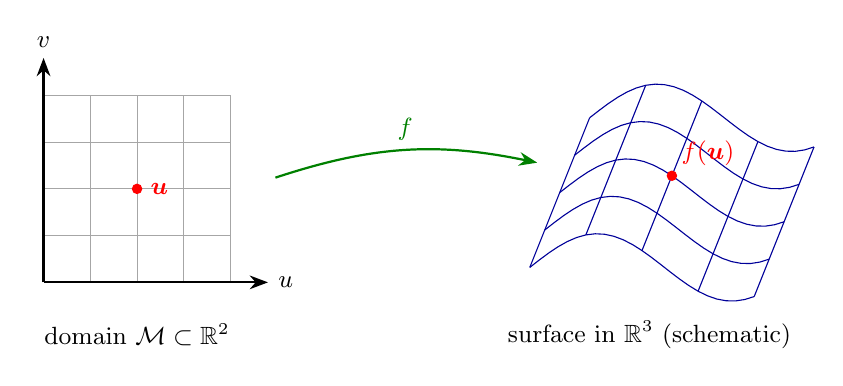
\begin{tikzpicture}[font=\small,>=Stealth,scale=0.95]
\begin{scope}
\foreach \u in {0,0.25,0.5,0.75,1}{\draw[gray!70] (2.5*\u,0)--(2.5*\u,2.5); \draw[gray!70] (0,2.5*\u)--(2.5,2.5*\u);}
\draw[->,thick] (0,0)--(3,0) node[right] {$u$}; \draw[->,thick] (0,0)--(0,3) node[above] {$v$};
\fill[red] (1.25,1.25) circle (2pt); \node[right,red] at (1.3,1.25) {$\vu$};
\node at (1.25,-0.7) {domain $\M\subset\R^2$};
\end{scope}
\begin{scope}[xshift=6.5cm,yshift=0.2cm]
\foreach \u in {0,0.25,0.5,0.75,1}{\draw[blue!60!black] plot[domain=0:1,samples=25,variable=\t] ({3*\u+0.8*\t},{2*\t+0.45*sin(300*\u)});}
\foreach \v in {0,0.25,0.5,0.75,1}{\draw[blue!60!black] plot[domain=0:1,samples=25,variable=\t] ({3*\t+0.8*\v},{2*\v+0.45*sin(300*\t)});}
\fill[red] (1.9,1.225) circle (2pt); \node[above right,red] at (1.9,1.225) {$f(\vu)$};
\node at (1.6,-0.9) {surface in $\R^3$ (schematic)};
\end{scope}
\draw[->,thick,green!50!black] (3.1,1.4) to[bend left=15] node[above] {$f$} (6.6,1.6);
\end{tikzpicture}
\includegraphics[width=0.75\textwidth]{tex/EAI02/parametric_surface.png}
\caption{A parametrization warps a flat domain into a surface: grid lines of $(u,v)$ become curves on the surface, and neighbouring parameters stay neighbouring.}
\end{figure}

\begin{example}[Analytic examples]
The saddle $f((u,v))=(u,\,v,\,v^2-u^2)$; and the trefoil-knot tube of slide 38:
\begin{lstlisting}
def trefoil(u, v):
    # r is just a float scale factor
    x = r * np.sin(3*u) / (2 + np.cos(v))
    y = r * (np.sin(u) + 2*np.sin(2*u)) / (2 + np.cos(v + np.pi*2/3))
    z = r/2 * (np.cos(u) - 2*np.cos(2*u)) * (2 + np.cos(v)) * (2 + np.cos(v + np.pi*2/3)) / 4
\end{lstlisting}
\end{example}

\begin{definition}[B\'ezier surface]
With $(N+1)(M+1)$ control points $\vk_{i,j}\in\R^3$,
\[
f((u,v))=\sum_{i=0}^{N}\sum_{j=0}^{M}B_i^N(u)\,B_j^M(v)\,\vk_{i,j},\qquad B_i^N(u)=\binom{N}{i}u^i(1-u)^{N-i}.
\]
Here $N$ and $M$ are polynomial \emph{degrees}, not counts. The control points determine a smooth surface in 3D; B\'ezier patches are commonly used for designing meshes.
\end{definition}
\begin{figure}[H]
\centering
\includegraphics[width=0.75\textwidth]{tex/EAI02/bezier_surface.png}
\caption{A B\'ezier surface}
\end{figure}

\begin{example}[The bilinear patch, $N=M=1$]
$B_0^1(u)=1-u$, $B_1^1(u)=u$, so $f=(1-u)(1-v)\vk_{00}+(1-u)v\,\vk_{01}+u(1-v)\vk_{10}+uv\,\vk_{11}$. With $\vk_{00}=(0,0,0)$, $\vk_{10}=(1,0,0)$, $\vk_{01}=(0,1,0)$, $\vk_{11}=(1,1,1)$: $f(0.5,0.5)=\tfrac14\big[(1,0,0)+(0,1,0)+(1,1,1)\big]=(0.5,0.5,0.25)$.
\end{example}

\begin{intuition}
Control points act like a coarse cage of pins: move a pin and the smooth sheet follows. The surface is a weighted average of the pins, with weights (Bernstein polynomials) that sum to one, so it stays inside the convex hull of the cage. That is why the same $(N+1)(M+1)$ numbers describe an entire smooth surface no matter how finely you later sample it.
\end{intuition}

\subsection{Parametric Surfaces --- Pros and Cons \slides{slide 41}}
\begin{itemize}[nosep]
\item \textbf{Sampling is easy:} pick $\vu$, evaluate $f$.
\item \textbf{Computation in the domain:} neighbours, texture coordinates and so on are just nearby $\vu$ values.
\item \textbf{``Is $\vq$ inside?'' is hard:} you would have to search for the $\vu$ whose $f(\vu)$ is closest to $\vq$, an optimization problem.
\item \textbf{Rendering is hard:} a ray hits the surface where $\vo+t\vd=f(\vu)$, a nonlinear system in $(t,\vu)$. In practice you convert to a mesh first.
\end{itemize}

\begin{intuition}
Generating is a \emph{forward} computation (plug in, read off); testing or intersecting needs the \emph{inverse} of $f$, which is generally not available in closed form. The price of the parametrization is also its topology: the surface has whatever topology $\M$ has (a sphere domain can only give sphere-like shapes).
\end{intuition}

% =====================================================================
\section{Surface Representations \slides{slide 42}}
% =====================================================================

Points, meshes and parametric surfaces all describe the ``skin'' of an object, and none of them can turn a torus into a sphere continuously. So what can we do?

\begin{intuition}
All three fix the topology in their data (the connectivity $F$, the domain $\M$, or the absence of connectivity). To let shapes change topology smoothly, one needs a representation that assigns a value to \emph{every point of space} rather than tracking the skin.
\end{intuition}

% =====================================================================
\section{Volume Representations \slides{slides 43--46}}
% =====================================================================

Volume representations give a value to every point in space.

\subsection{Voxelized 3D \slides{slides 44--46}}
\begin{definition}[Voxel grid]
A voxel grid is a discretized representation of the space demarcated via cuboid endpoints $(x_{\min},y_{\min},z_{\min})$ and $(x_{\max},y_{\max},z_{\max})$: a $W\times H\times D$ array $V[i,j,k]\in[0,1]$ storing the occupancy (or probability of occupancy) of each cell.
\end{definition}

\begin{figure}[H]
\centering
\includegraphics[width=0.75\textwidth]{tex/EAI02/voxel_grid.png}
\caption{A $4\times4\times4$ voxel grid inside a cuboid; shaded cells are occupied.}
\end{figure}

\textbf{Coding tip:} disentangle \emph{grid coordinates} from the \emph{spatial extent in the world}. One common convention: cell size $h=(x_{\max}-x_{\min})/W$ along $x$, and cell $i$ has its centre at $x_{\min}+(i+\tfrac12)h$; the same for $y,z$. For $x_{\min}=-1.5$, $x_{\max}=1.5$, $W=128$: $h\approx0.0234$, and the point $x=0.3$ falls in cell $i=\lfloor(0.3+1.5)/h\rfloor=76$.

Because the representation is ``image-like'', \emph{convolutions} can be used for processing and generation. It is a generic way to represent shapes \emph{across topologies}: the sphere, the torus and the cow of slide 45 all use the same array shape, and topology is just which cells are switched on. A fixed-size output is exactly what networks like.

\subsubsection*{Resolution is expensive \slides{slide 46}}
It is computationally challenging to scale resolution ($32^3,64^3,128^3,256^3$ on the slide). Worse, the surface passes through only about $n^2$ of the $n^3$ cells, so almost all the memory describes empty space or solid interior.

\begin{figure}[H]
\centering
\includegraphics[width=0.75\textwidth]{tex/EAI02/voxel_grid_resolution.png}
\caption{A rappresentation of how resolution affects surface detail. The surface passes through only about $n^2$ of the $n^3$ cells, so almost all the memory describes empty space or solid interior.}
\end{figure}

\begin{example}[Memory of a voxel grid]
\begin{center}
\begin{tabular}{rrrr}
\toprule
$n$ & cells $n^3$ & surface cells $\approx n^2$ & fraction $\approx 1/n$ \\
\midrule
32 & 32\,768 & 1\,024 & 3\% \\
64 & 262\,144 & 4\,096 & 1.6\% \\
128 & 2\,097\,152 & 16\,384 & 0.8\% \\
256 & 16\,777\,216 & 65\,536 & 0.4\% \\
\bottomrule
\end{tabular}
\end{center}
At one byte per cell, $256^3$ is 16\,MB (64\,MB with 32-bit floats) for a single object.
\end{example}

\begin{figure}[ht]
\centering
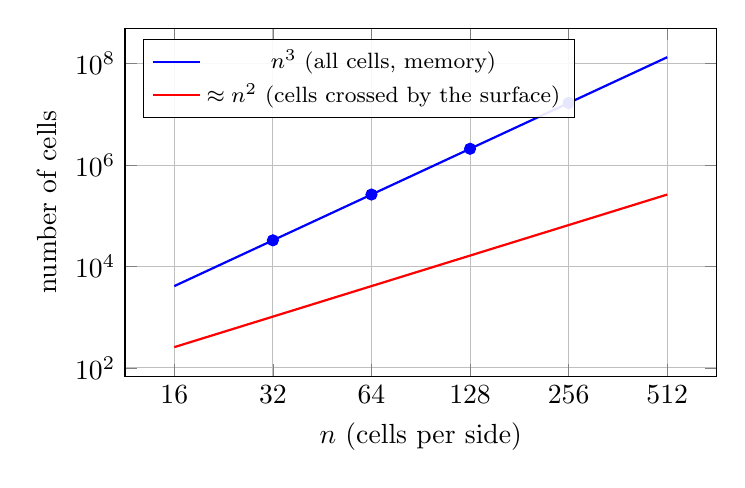
\begin{tikzpicture}
\begin{axis}[width=0.75\linewidth,height=6cm,xmode=log,ymode=log,xlabel={$n$ (cells per side)},ylabel={number of cells},
 xtick={16,32,64,128,256,512},xticklabels={16,32,64,128,256,512},grid=both,legend pos=north west,legend style={font=\footnotesize,fill=white,fill opacity=0.9,text opacity=1,draw opacity=1}]
\addplot[blue,thick,domain=16:512,samples=2] {x^3}; \addlegendentry{$n^3$ (all cells, memory)}
\addplot[red,thick,domain=16:512,samples=2] {x^2}; \addlegendentry{$\approx n^2$ (cells crossed by the surface)}
\addplot[only marks,mark=*,blue] coordinates {(32,32768)(64,262144)(128,2097152)(256,16777216)};
\end{axis}
\end{tikzpicture}
\caption{Doubling the resolution multiplies memory by 8 but the useful (surface) part only by 4.}
\end{figure}

\begin{intuition}
A voxel grid is a bookkeeping device: it pays the same for air as for the object. Doubling the resolution costs $8\times$ more memory but only $4\times$ more surface. The benefit is simplicity: any topology, fixed size, convolutions apply. The cost is that fine detail is very expensive, which motivates adaptive versions (octrees, slide 68) and continuous fields (next section).
\end{intuition}

% =====================================================================
\section{Implicit Surfaces \slides{slides 47--62}}
% =====================================================================

\subsection{Implicit surfaces \slides{slide 47}}
\begin{definition}[Implicit surface]
A surface is the \emph{zero level set} of a scalar field $f:\R^3\to\R$:
\[
\Surf=\{\vx\in\R^3\mid f(\vx)=0\}.
\]
The sign tells the side: $f(\vx)<0$ inside, $f(\vx)>0$ outside (one convention, used for the rest of the lecture).
\end{definition}

\subsection{Generate vs Test \slides{slide 48}}
The unit circle, written both ways:
\begin{center}
\begin{tabular}{L{3.2cm}L{5.4cm}L{5.4cm}}
\toprule
 & \textbf{Parametric} & \textbf{Implicit}\\
\midrule
Definition & $g(u)=(\cos u,\sin u)$, $u\in[0,2\pi)$ & $f(x,y)=x^2+y^2-1$\\
Give me 100 points on it & easy: evaluate $g$ at 100 values of $u$ & hard: you have to search for zeros\\
Is $(0.5,0.5)$ inside? & hard: no direct test & easy: $f=-0.5<0$, so inside\\
\bottomrule
\end{tabular}
\end{center}
Parametric representations \emph{generate} points; implicit representations \emph{test} points.

\begin{figure}[ht]
\centering
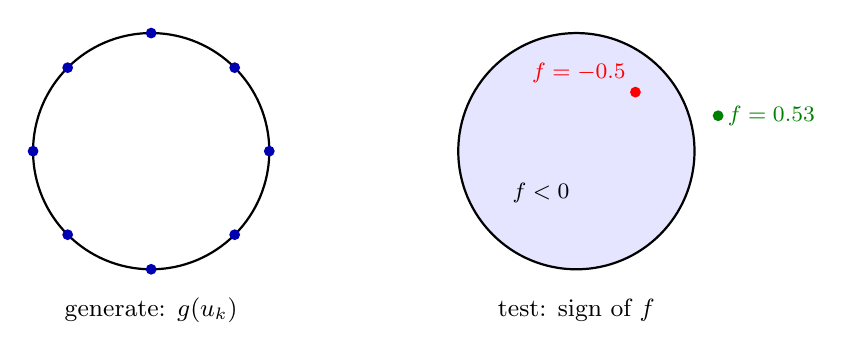
\begin{tikzpicture}[font=\small,scale=1.5]
\draw[thick] (0,0) circle (1);
\foreach \i in {0,...,7}{\fill[blue!70!black] (45*\i:1) circle (1.3pt);}
\node at (0,-1.35) {generate: $g(u_k)$};
\begin{scope}[xshift=3.6cm]
\fill[blue!10] (0,0) circle (1);
\draw[thick] (0,0) circle (1);
\fill[red] (0.5,0.5) circle (1.3pt) node[above left,font=\footnotesize] {$f=-0.5$};
\fill[green!50!black] (1.2,0.3) circle (1.3pt) node[right,font=\footnotesize] {$f=0.53$};
\node[font=\footnotesize] at (-0.3,-0.35) {$f<0$};
\node at (0,-1.35) {test: sign of $f$};
\end{scope}
\end{tikzpicture}
\caption{Left: the parametric circle produces points. Right: the implicit circle classifies any point by the sign of $f$.}
\end{figure}

\begin{intuition}
Parametric $\approx$ a machine that \emph{prints} surface points; implicit $\approx$ a \emph{bouncer} that checks tickets. Printing 100 points is trivial with the printer and awkward with the bouncer (you have to hunt for the zeros); checking a single point is trivial with the bouncer and awkward with the printer (you must invert $g$).
\end{intuition}

\subsection{Implicit Surfaces: Examples \slides{slide 49}}
Simple functions can give concise representations of complex shapes:
\begin{align*}
\text{sphere:}\quad & f(x,y,z)=x^2+y^2+z^2-1,\\
\text{torus:}\quad & f(x,y,z)=(x^2+y^2+z^2+R^2-a^2)^2-4R^2(x^2+y^2),\\
\text{quartic (blob with a hole):}\quad & f(x,y,z)=x^4+y^4+z^4+2x^2y^2+2x^2z^2\\
& \qquad\quad{}+2y^2z^2+8xyz-10x^2-10y^2-10z^2+20.
\end{align*}

\begin{figure}[H]
\centering
\includegraphics[width=0.75\textwidth]{tex/EAI02/implicit_examples.png}
\caption{Implicit surfaces: sphere, torus, and a quartic with a hole. The last one is a single polynomial of degree 4, yet it has a hole in it.}
\end{figure}

\subsection{When a Field Defines a Surface \slides{slide 50}}
Not every field defines a surface. Four test cases (with $r=\norm{\vx}$):
\begin{center}
\begin{tabular}{lll}
\toprule
$f(\vx)$ & zero set & a surface?\\
\midrule
$\norm{\vx}-1$ & unit sphere & yes\\
$\norm{\vx}^2+1$ & empty & no, there is nothing there\\
$\norm{\vx}^2$ & the origin & no, a single point\\
$(\norm{\vx}-1)^2$ & unit sphere & no: $f\ge0$ everywhere, so no inside, and $\nabla f=0$ on it\\
\bottomrule
\end{tabular}
\end{center}

\begin{proposition}[When $f$ defines a surface]
$f$ must change sign across $\Surf$, and $\nabla f\ne 0$ on $\Surf$. (If $f$ is continuously differentiable and $\nabla f\neq0$ at every zero of $f$, the implicit function theorem shows that $\Surf$ is locally the graph of a smooth function, i.e.\ a smooth surface.)
\end{proposition}

\begin{figure}[ht]
\centering
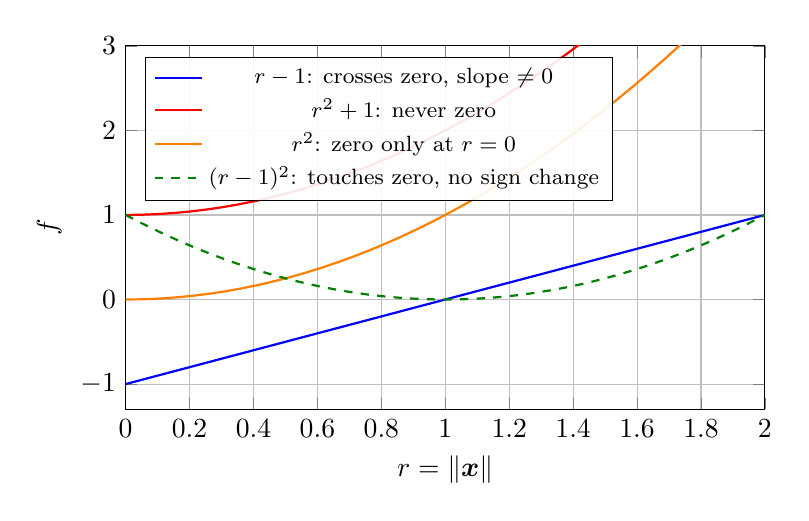
\begin{tikzpicture}
\begin{axis}[width=0.8\linewidth,height=6.2cm,xlabel={$r=\norm{\vx}$},ylabel={$f$},xmin=0,xmax=2,ymin=-1.3,ymax=3,grid=both,legend pos=north west,legend style={font=\footnotesize,fill=white,fill opacity=0.9,text opacity=1,draw opacity=1}]
\addplot[thick,blue,domain=0:2,samples=2] {x-1}; \addlegendentry{$r-1$: crosses zero, slope $\ne0$}
\addplot[thick,red,domain=0:2,samples=40] {x^2+1}; \addlegendentry{$r^2+1$: never zero}
\addplot[thick,orange,domain=0:2,samples=40] {x^2}; \addlegendentry{$r^2$: zero only at $r=0$}
\addplot[thick,green!50!black,dashed,domain=0:2,samples=40] {(x-1)^2}; \addlegendentry{$(r-1)^2$: touches zero, no sign change}
\end{axis}
\end{tikzpicture}
\caption{Radial profiles of the four candidate fields. Only the first one changes sign at the unit sphere with a non-zero slope.}
\end{figure}

\begin{intuition}
A surface is where the field \emph{crosses} zero, like the shoreline where altitude crosses sea level. A field that only touches zero (the last row) gives a double root: no ``inside'', no well-defined normal. A field that never reaches zero gives nothing.
\end{intuition}

\subsection{Normals for Free \slides{slide 51}}
\begin{lemma}[Normal of an implicit surface]
The gradient is perpendicular to the level sets, so on the surface
\[
\vn(\vx)=\frac{\nabla f(\vx)}{\norm{\nabla f(\vx)}}.
\]
It points toward increasing $f$, which by our convention is \emph{outward}.
\end{lemma}
\begin{proof}
Let $\gamma(t)$ be any curve lying in $\Surf$. Then $f(\gamma(t))=0$ for all $t$; differentiating, $\nabla f(\gamma(t))\cdot\gamma'(t)=0$, so $\nabla f$ is orthogonal to every tangent direction of the surface.
\end{proof}

For the sphere, $\nabla f=2\vx$ and $\vn=\vx/\norm{\vx}$. With automatic differentiation the normals of \emph{any} differentiable $f$ (an MLP, say) come for free:
\begin{lstlisting}
x = pts.clone().requires_grad_(True)            # (N, 3) points
v = f(x)                                        # any differentiable f, e.g. an MLP
g, = torch.autograd.grad(v.sum(), x)
n = g / g.norm(dim=-1, keepdim=True)            # (N, 3) unit normals
\end{lstlisting}

\begin{figure}[ht]
\centering
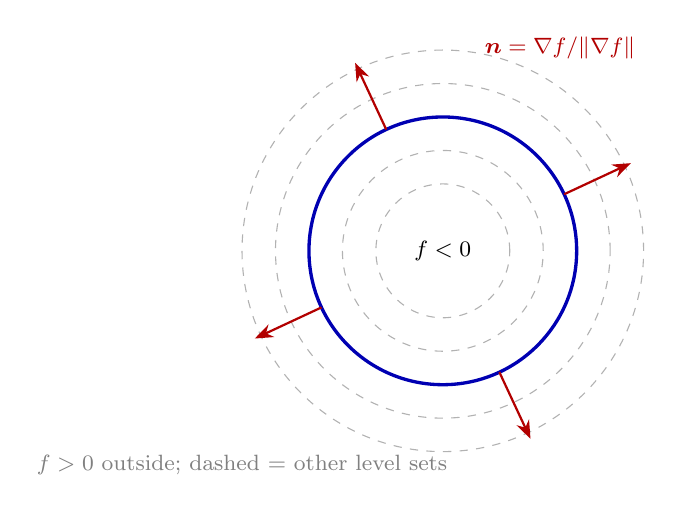
\begin{tikzpicture}[font=\small,>=Stealth,scale=1.7]
\foreach \r in {0.5,0.75,1.25,1.5}{\draw[gray!60,dashed] (0,0) circle (\r);}
\draw[very thick,blue!70!black] (0,0) circle (1);
\foreach \a in {25,115,205,295}{\draw[->,thick,red!70!black] (\a:1) -- (\a:1.55);}
\node[red!70!black,font=\footnotesize] at (60:1.75) {$\vn=\nabla f/\norm{\nabla f}$};
\node[font=\footnotesize] at (0,0) {$f<0$};
\node[font=\footnotesize,gray] at (-1.5,-1.6) {$f>0$ outside; dashed = other level sets};
\end{tikzpicture}
\caption{The gradient of $f$ is orthogonal to the level sets and points toward larger $f$, i.e.\ out of the shape.}
\end{figure}

\begin{intuition}
Picture $f$ as terrain height and the surface as the zero contour line. The gradient points straight uphill, perpendicular to any contour line: that is the normal. No separate normal array has to be stored or kept consistent, unlike the per-face orientation of a mesh.
\end{intuition}

\subsection{Boolean Operations \slides{slide 52}}
\begin{proposition}[Booleans via $\min$ and $\max$]
With $f<0$ inside,
\[
f_{A\cup B}=\min(f_A,f_B),\qquad f_{A\cap B}=\max(f_A,f_B),\qquad f_{A\setminus B}=\max(f_A,-f_B).
\]
\end{proposition}
\begin{proof}
$\vx\in A\cup B\iff f_A(\vx)<0$ or $f_B(\vx)<0\iff\min(f_A,f_B)<0$. Likewise $\vx\in A\cap B\iff f_A<0$ and $f_B<0\iff\max(f_A,f_B)<0$. For $A\setminus B=A\cap B^{c}$, the complement of $B$ is described (up to its boundary) by $-f_B<0$, so $\max(f_A,-f_B)<0$.
\end{proof}

\begin{figure}[ht]
\centering
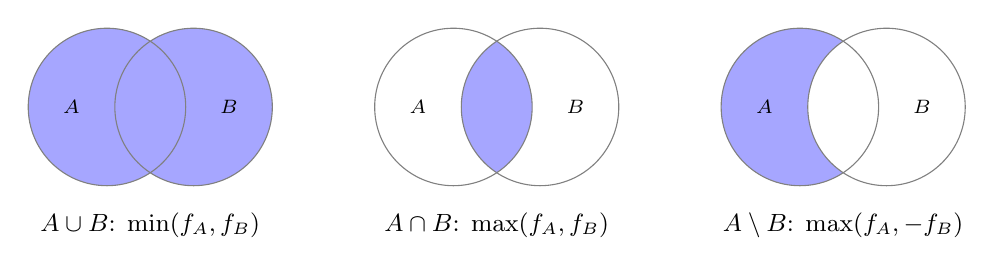
\begin{tikzpicture}[font=\small]
\foreach \dx/\k/\t in {0/0/{$A\cup B$: $\min(f_A,f_B)$},4.4/1/{$A\cap B$: $\max(f_A,f_B)$},8.8/2/{$A\setminus B$: $\max(f_A,-f_B)$}}{
 \begin{scope}[xshift=\dx cm]
 \ifnum\k=0 \fill[blue!35] (0,0) circle (1) (1.1,0) circle (1); \fi
 \ifnum\k=1 \begin{scope}\clip (0,0) circle (1); \fill[blue!35] (1.1,0) circle (1);\end{scope} \fi
 \ifnum\k=2 \begin{scope}\clip (0,0) circle (1); \begin{scope}[even odd rule]\clip (-3,-3) rectangle (4,3) (1.1,0) circle (1); \fill[blue!35] (-3,-3) rectangle (4,3);\end{scope}\end{scope} \fi
 \draw[gray] (0,0) circle (1); \draw[gray] (1.1,0) circle (1);
 \node at (-0.45,0) {\scriptsize $A$}; \node at (1.55,0) {\scriptsize $B$};
 \node at (0.55,-1.5) {\t};
 \end{scope}
}
\end{tikzpicture}
\caption{2D versions of the three Boolean operations (blue = result).}
\end{figure}

\begin{intuition}
``Inside the union'' means ``inside at least one'': the most negative of the two values decides, hence $\min$. ``Inside the intersection'' needs both, so the \emph{least} negative value decides: $\max$. Subtraction is intersection with the outside of $B$, and flipping the sign of $f_B$ swaps inside and outside. The \emph{sign} of the result is always correct; the magnitude near sharp creases is not guaranteed to remain an exact distance (see the SDF discussion next).
\end{intuition}

\subsection{Many Functions, One Surface \slides{slide 53}}
The surface does not fix $f$: many different fields have the same zero set. So one can choose an $f$ that is useful \emph{away} from the surface.

\subsection{Signed Distance Function \slides{slides 54--58}}
\begin{definition}[Signed distance function (SDF)]
\[
f(\vx)=\begin{cases}-\dist(\vx,\Surf)&\vx\text{ inside}\\ +\dist(\vx,\Surf)&\vx\text{ outside}\end{cases},\qquad \dist(\vx,\Surf)=\min_{\vy\in\Surf}\norm{\vx-\vy}.
\]
\end{definition}

Which of the fields of slide 55 are SDFs? $x^2+y^2+z^2-1$ and the quartic of slide 49: \emph{neither}!

\begin{proposition}[Eikonal condition]\label{prop:eikonal}
An SDF satisfies $\norm{\nabla f}=1$ (wherever it is differentiable).
\end{proposition}
\begin{proof}
Take a small step of length $\delta$ from a point. In \emph{any} direction the distance to the surface changes by at most $\delta$; stepping straight away from the closest surface point it changes by exactly $\delta$. So the steepest slope of $f$ is exactly one.
\end{proof}

\begin{example}
$f=\norm{\vx}-1$: $\nabla f=\vx/\norm{\vx}$, $\norm{\nabla f}=1$, an SDF. $f=\norm{\vx}^2-1$: $\nabla f=2\vx$, $\norm{\nabla f}=2\norm{\vx}\ne1$, not an SDF.
\end{example}

\begin{figure}[ht]
\centering
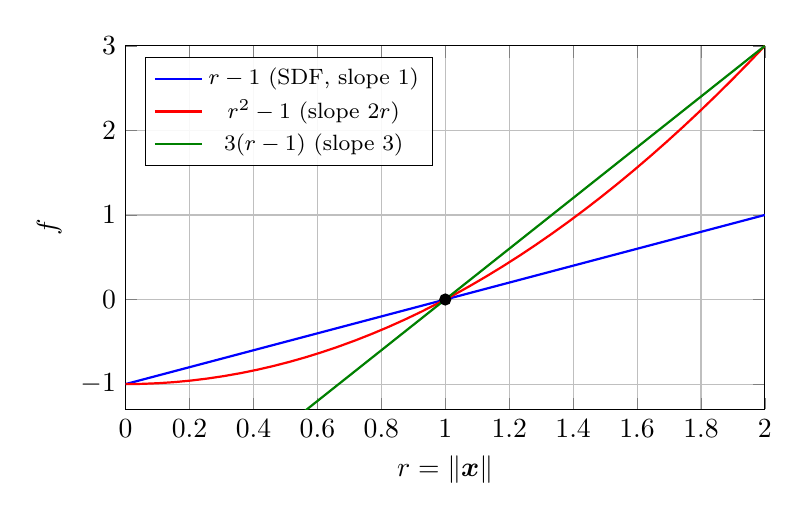
\begin{tikzpicture}
\begin{axis}[width=0.8\linewidth,height=6.2cm,xlabel={$r=\norm{\vx}$},ylabel={$f$},xmin=0,xmax=2,ymin=-1.3,ymax=3,grid=both,legend pos=north west,legend style={font=\footnotesize,fill=white,fill opacity=0.9,text opacity=1,draw opacity=1}]
\addplot[thick,blue,domain=0:2,samples=2] {x-1}; \addlegendentry{$r-1$ (SDF, slope 1)}
\addplot[thick,red,domain=0:2,samples=40] {x^2-1}; \addlegendentry{$r^2-1$ (slope $2r$)}
\addplot[thick,green!50!black,domain=0:2,samples=2] {3*(x-1)}; \addlegendentry{$3(r-1)$ (slope 3)}
\addplot[only marks,mark=*,black] coordinates {(1,0)};
\end{axis}
\end{tikzpicture}
\caption{Three fields with the same zero set (the unit sphere, $r=1$). Only the slope-one profile is a signed distance function.}
\end{figure}

\begin{intuition}
The eikonal condition says ``the field grows like a ruler as you walk away from the surface''. An SDF is the most \emph{honest} field: its value literally is the distance to the surface. The other fields agree on \emph{where} the surface is but exaggerate or shrink the distances; $r^2-1$ overstates by the factor $r+1$ at radius $r$.
\end{intuition}

\paragraph{Why honesty matters: safe steps \slides{slides 57--58}.}
\begin{proposition}[Safe step]
If $f$ is an SDF, the ball of radius $\abs{f(\vx)}$ around $\vx$ contains no surface point in its interior. Hence a ray can safely advance by $\abs{f(\vx)}$. If $f$ overstates the distance, the ball can cross the surface and stepping by $f$ can \emph{jump through} it.
\end{proposition}
\begin{proof}
By definition $\abs{f(\vx)}=\dist(\vx,\Surf)$, the radius of the largest ball around $\vx$ that avoids $\Surf$. For a non-SDF field the ball of radius $\abs{f}$ can be larger than $\dist(\vx,\Surf)$ and then contains surface points.
\end{proof}

\begin{example}[Slides 57--58, $\vx$ at $r\approx2.67$]
For $f=r^2-1$: $f=6.14$, true distance $1.67$, $\norm{\nabla f}=5.34$: the circle of radius $\abs f$ crosses the surface. For an SDF at the same point the ball of radius $r-1=1.67$ touches the surface without crossing.
\end{example}

\begin{figure}[ht]
\centering
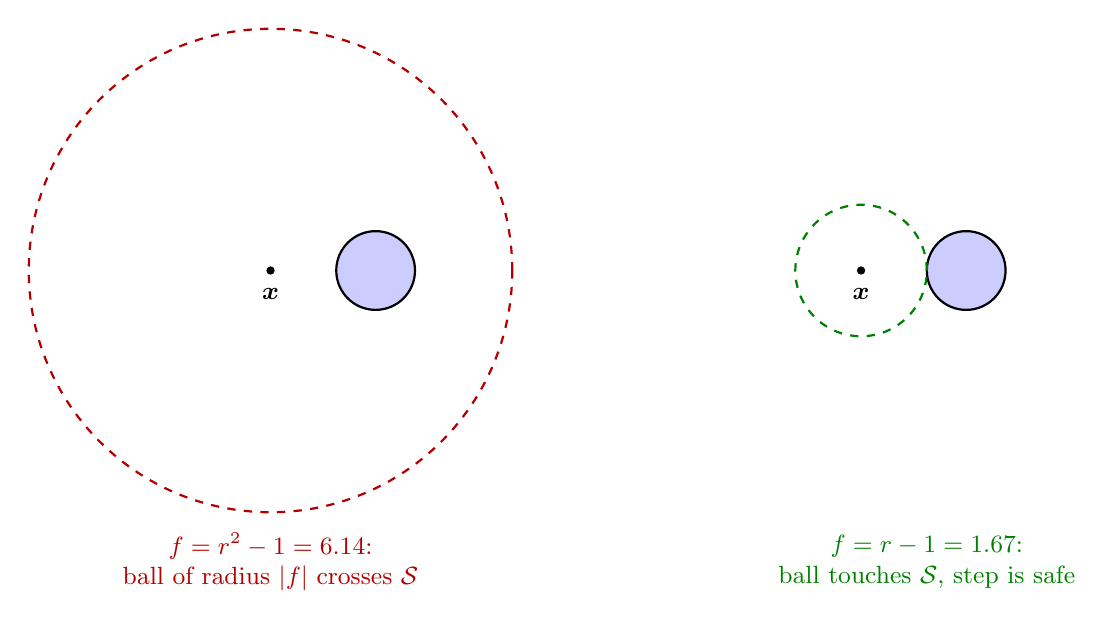
\begin{tikzpicture}[font=\small,scale=0.5]
\begin{scope}
\fill[blue!20] (0,0) circle (1); \draw[thick] (0,0) circle (1);
\draw[dashed,red!70!black,thick] (-2.67,0) circle (6.14);
\fill (-2.67,0) circle (3pt); \node[below] at (-2.67,-0.2) {$\vx$};
\node[red!70!black,align=center] at (-2.67,-7.4) {$f=r^2-1=6.14$:\\ball of radius $|f|$ crosses $\Surf$};
\end{scope}
\begin{scope}[xshift=15cm]
\fill[blue!20] (0,0) circle (1); \draw[thick] (0,0) circle (1);
\draw[dashed,green!50!black,thick] (-2.67,0) circle (1.67);
\fill (-2.67,0) circle (3pt); \node[below] at (-2.67,-0.2) {$\vx$};
\node[green!50!black,align=center] at (-1,-7.4) {$f=r-1=1.67$:\\ball touches $\Surf$, step is safe};
\end{scope}
\end{tikzpicture}
\caption{The same point $\vx$ with two fields that define the same sphere. Left: stepping by $f=r^2-1$ overshoots. Right: an SDF gives the largest safe step.}
\end{figure}

\begin{algorithm}[Sphere tracing / ray marching an SDF]
Given a ray $\vo+t\vd$ ($\norm{\vd}=1$) and an SDF $f$: set $t\leftarrow0$; repeat $t\leftarrow t+f(\vo+t\vd)$ until $f<\varepsilon$ (hit) or $t$ exceeds a maximum (miss).
\end{algorithm}

\begin{figure}[ht]
\centering
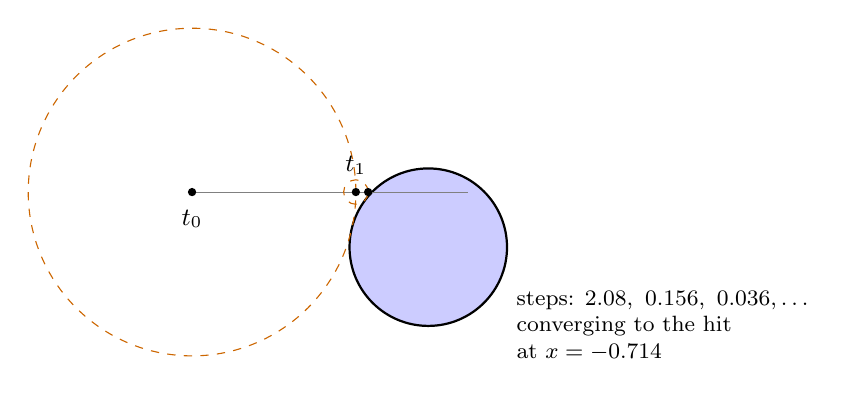
\begin{tikzpicture}[font=\small,>=Stealth]
\fill[blue!20] (0,0) circle (1); \draw[thick] (0,0) circle (1);
\draw[gray] (-3,0.7) -- (0.5,0.7);
\draw[dashed,orange!80!black] (-3,0.7) circle (2.0806);
\draw[dashed,orange!80!black] (-0.9194,0.7) circle (0.1556);
\draw[dashed,orange!80!black] (-0.7638,0.7) circle (0.0361);
\foreach \x in {-3,-0.9194,-0.7638}{\fill (\x,0.7) circle (1.5pt);}
\node[below] at (-3,0.6) {$t_0$}; \node[above] at (-0.9194,0.8) {$t_1$};
\node[align=left,font=\footnotesize] at (3,-1.0) {steps: $2.08,\ 0.156,\ 0.036,\dots$\\converging to the hit\\at $x=-0.714$};
\end{tikzpicture}
\caption{Sphere tracing a horizontal ray at height $0.7$ against the unit sphere: each step is the SDF value, the radius of the empty ball.}
\end{figure}

\begin{intuition}
It is like walking through fog toward a wall with a distance meter: if the meter never lies (SDF) you can always walk the displayed distance without hitting the wall, and the steps shrink as you approach. A meter that overstates makes you walk into and through the wall. This is why the table on slide 66 lists ``ray marching'' as the way to render implicit surfaces.
\end{intuition}

\subsection{Storing a Field on a Grid \slides{slide 59}}
Store samples $F[i,j,k]=f(\vx_{ijk})$ at the grid points and interpolate in between: the same data structure as a voxel grid, but holding \emph{signed distances} rather than occupancy. A \emph{TSDF} keeps values only near the surface and clamps them to $\pm\tau$ elsewhere, $f_\tau=\clamp(f,-\tau,\tau)$; it is the standard way to fuse many depth maps into one model, as in KinectFusion.
\begin{lstlisting}
xs = np.linspace(-1.5, 1.5, 128)
X, Y, Z = np.meshgrid(xs, xs, xs, indexing="ij")
F = np.sqrt(X**2 + Y**2 + Z**2) - 1.0           # unit-sphere SDF on a 128^3 grid
\end{lstlisting}

\begin{intuition}
The grid now stores \emph{how far} each cell is from the surface instead of \emph{whether} it is occupied. Values change smoothly across the surface, so interpolation places the surface at sub-voxel accuracy, and the clamped version stores only what matters: a thin shell around the surface.
\end{intuition}

\subsection{Storing a Field in a Network \slides{slide 60}}
$\{\vx\mid f_\theta(\vx)=0\}$, with $f_\theta$ a small MLP (three numbers in, one out). Two requirements: $f_\theta(\vx_i)\approx0$ on the data points (the surface passes through the data), and $\norm{\nabla f_\theta(\vx)}\approx1$ everywhere (it behaves like an SDF). Resolution is not tied to a grid.

\begin{figure}[H]
\centering
\includegraphics[width=0.75\textwidth]{tex/EAI02/implicit_network.png}
\caption{A small MLP can represent a continuous field $f_\theta$, whose zero set is the surface.}
\end{figure}

\begin{example}[One way to write the two requirements as a loss]
$\mathcal L(\theta)=\frac1N\sum_i\abs{f_\theta(\vx_i)}+\lambda\,\mathbb E_{\vx}\big[(\norm{\nabla f_\theta(\vx)}-1)^2\big]$. The first term pulls the zero set through the samples; the second is the eikonal penalty of Proposition~\ref{prop:eikonal}.
\end{example}

\begin{intuition}
The network is a \emph{compressed}, resolution-free grid: query it at any point, at any density. The eikonal penalty is what stops the network from producing an arbitrary function that merely vanishes on the data.
\end{intuition}

\subsection{From Implicit Surface to Mesh \slides{slide 61}}

\begin{figure}[H]
\centering
\includegraphics[width=0.75\textwidth]{tex/EAI02/marching_squares.png}
\caption{Marching squares (the 2D version of marching cubes) in one cell. The blue corners are inside ($f<0$),the white corners are outside ($f>0$). The dotted line is the true surface; the orange line is the interpolated surface from marching squares.}
\end{figure}
\begin{algorithm}[Marching cubes]\label{alg:mc}
\textbf{1.}~Evaluate $f$ on a grid (analytic, a TSDF, or a network).\\
\textbf{2.}~Find the cells whose corners differ in sign.\\
\textbf{3.}~On each such edge $[\va,\vb]$, place a vertex at the zero crossing
$p=\va+t(\vb-\va)$ with $t=\dfrac{f(\va)}{f(\va)-f(\vb)}$.\\
\textbf{4.}~In 3D, join the vertices with a lookup table on the corner signs: $2^8$ cases per cube.
\end{algorithm}

\begin{lstlisting}
from skimage.measure import marching_cubes
h = xs[1] - xs[0]                                # voxel size, from the grid above
verts, faces, normals, _ = marching_cubes(F, level=0.0, spacing=(h, h, h))
verts += xs[0]                                   # grid -> world coordinates
\end{lstlisting}

\begin{figure}[ht]
\centering
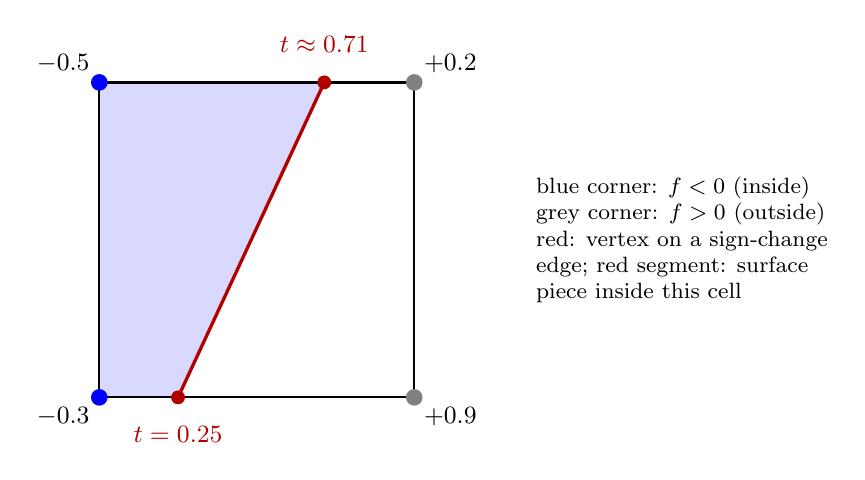
\begin{tikzpicture}[font=\small]
\fill[blue!15] (0,0)--(1,0)--(2.857,4)--(0,4)--cycle;
\draw[thick] (0,0) rectangle (4,4);
\draw[very thick,red!70!black] (1,0)--(2.857,4);
\fill[blue] (0,0) circle (3pt); \fill[blue] (0,4) circle (3pt);
\fill[gray] (4,0) circle (3pt); \fill[gray] (4,4) circle (3pt);
\node[below left] at (0,0) {$-0.3$}; \node[below right] at (4,0) {$+0.9$};
\node[above left] at (0,4) {$-0.5$}; \node[above right] at (4,4) {$+0.2$};
\fill[red!70!black] (1,0) circle (2.5pt); \fill[red!70!black] (2.857,4) circle (2.5pt);
\node[below,red!70!black] at (1,-0.25) {$t=0.25$}; \node[above,red!70!black] at (2.857,4.25) {$t\approx0.71$};
\node[align=left,font=\footnotesize] at (7.4,2) {blue corner: $f<0$ (inside)\\grey corner: $f>0$ (outside)\\red: vertex on a sign-change\\edge; red segment: surface\\piece inside this cell};
\end{tikzpicture}
\caption{Marching squares (the 2D version of marching cubes) in one cell. On the bottom edge $t=\frac{-0.3}{-0.3-0.9}=0.25$; on the top edge $t=\frac{-0.5}{-0.5-0.2}\approx0.71$. The left and right edges have no sign change, hence no vertex.}
\end{figure}

\begin{intuition}
Marching cubes is ``connect the dots along the shoreline'': the corner signs say which cell edges the coastline crosses; linear interpolation of $f$ along that edge says \emph{where} (a corner with a small $|f|$ is close to the surface, so the vertex sits close to it). This is the bridge from implicit to mesh, which is what GPUs render.
\end{intuition}

\subsection{Implicit Surfaces: Summary \slides{slide 62}}
\begin{center}
\begin{tabular}{L{6.6cm}L{6.6cm}}
\toprule
\textbf{Easy} & \textbf{Hard}\\
\midrule
inside or outside: the sign of $f$ & getting points on the surface\\
any topology, changing continuously & no direct rasterization\\
booleans: a $\min$ or a $\max$ & an arbitrary $f$ may define nothing\\
normals: $\nabla f$ & \\
\bottomrule
\end{tabular}
\end{center}
The mirror image of parametric surfaces.

% =====================================================================
\section{Boundary vs Volumetric Representations \slides{slide 63}}
% =====================================================================
Slide 63 summarizes the two families: \emph{boundary} representations for shapes (point clouds, meshes, parametric surfaces) and \emph{volumetric} representations for shapes (voxels, implicit fields).

% =====================================================================
\section{Density Fields \slides{slides 64--65}}
% =====================================================================
\subsection{Density fields \slides{slide 64}}
Occupancy asks ``is this point inside?''; density asks ``how opaque is this point?''.

\begin{figure}[H]
\centering
\includegraphics[width=0.75\textwidth]{tex/EAI02/density_field.png}
\caption{Two images examples}
\end{figure}
\begin{definition}[Density field]
A density field assigns $\sigma(\vx)\in\R^+$ (or $\sigma[i,j,k]\in\R^+$ on a grid); $\sigma(\vx)\ge0$ says how much light is absorbed per unit length at $\vx$.
\end{definition}

There is no notion of a surface: e.g.\ $\sigma(\vx)=0.1$ everywhere represents a semi-transparent fluid. Typical examples on the slide: smoke and CT-scan slices. The lecture will revisit this in more detail later (NeRF).

\begin{example}[Preview: how much light survives?]
If a beam crosses a slab of length $L$ of constant density $\sigma$, the fraction of light transmitted is $e^{-\sigma L}$ (absorption per unit length compounds multiplicatively). For $\sigma=0.1$ and $L=10$: $e^{-1}\approx0.37$. (This is a standard consequence of the ``absorbed per unit length'' reading; the slides develop it later.)
\end{example}

\subsection{Primitive-based Density Fields \slides{slide 65}}
\[
\sigma(\vx)=\sum_k w_k\exp\!\Big(-\tfrac12(\vx-\vmu_k)^{\!\top}\Sigma_k^{-1}(\vx-\vmu_k)\Big).
\]
These are \emph{hybrid} representations for primitive-induced density fields (blobs/Gaussians with weights $w_k$, centres $\vmu_k$, covariances $\Sigma_k$); the lecture will revisit them in more detail (differentiable Gaussian rendering).
\begin{figure}[H]
\centering
\includegraphics[width=0.75\textwidth]{tex/EAI02/density_fields_example.png}
\caption{Images examples of primitive-based density fields}
\end{figure}

\begin{intuition}
Instead of a grid of numbers, the density is a \emph{cloud of soft blobs}: each blob has a position, a size/orientation (via $\Sigma_k$) and a weight. The whole field can be edited by moving blobs, and only regions with blobs cost anything, so it avoids the ``pay for empty space'' problem of dense grids.
\end{intuition}

% =====================================================================
\section{So? \slides{slide 66}}
% =====================================================================
Slide 66 compares the representations side by side (its cells are colour-coded easy / possible with effort / hard; the colours do not survive in the text of the PDF, so the qualitative ratings appear in Section~\ref{sec:summary}, based on the earlier slides):

\begin{center}
\small
\renewcommand{\arraystretch}{1.25}
\setlength{\tabcolsep}{3pt}\begin{tabular}{L{2.2cm}L{2.4cm}L{2.3cm}L{2.4cm}L{2.1cm}L{2.5cm}}
\toprule
 & \textbf{Points on the surface} & \textbf{Inside or outside?} & \textbf{Continuous edits reach} & \textbf{Rendering} & \textbf{Typical use}\\
\midrule
\textbf{Point cloud} (array $N\times3$) & given & no surface & any point set & splats & sensors: LiDAR, RGB-D\\
\textbf{Mesh} ($V:N\times3$, $F:M\times3$) & sample triangles & count ray crossings & same wiring only & GPU rasterizer & graphics, games\\
\textbf{Parametric} ($f(\vu)$) & evaluate $f$ & search over $\vu$ & same topology only & via a mesh & CAD, design\\
\textbf{Voxels} (grid $W\times H\times D$) & marching cubes & look up the cell & any topology* & blocky & 3D CNNs, occupancy maps\\
\textbf{Implicit (SDF)} ($f(\vx)$: formula, grid, net) & marching cubes & sign of $f$ & any topology & ray marching & reconstruction, neural fields\\
\bottomrule
\end{tabular}
\end{center}
{\small * with occupancy probabilities, not $0$ or $1$.}

\begin{intuition}
\emph{No row wins every column: pick the representation for the task.} Need to shoot rays fast on a GPU? Mesh. Need to change topology or run inside/outside queries? Implicit. Data straight from a LiDAR? Points. Feeding a 3D CNN? Voxels.
\end{intuition}

% =====================================================================
\section{And many more\dots\ \slides{slides 67--71}}
% =====================================================================

\subsection{Octrees \slides{slide 68}}
Octrees are \emph{voxels with adaptive resolution}: surface-like efficiency for rendering and storage, volume-like efficiency for occupancy queries; but it is difficult to edit or predict the sparsity structure.

\begin{figure}[ht]
\centering
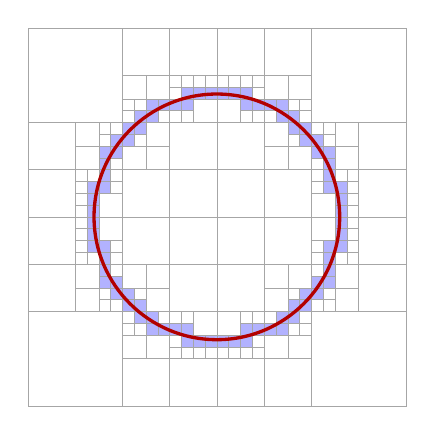
\begin{tikzpicture}[scale=2.4]
\fill[blue!30] (-0.5625,-0.4375) rectangle (-0.5000,-0.3750);
\fill[blue!30] (-0.6250,-0.3750) rectangle (-0.5625,-0.3125);
\fill[blue!30] (-0.6250,-0.3125) rectangle (-0.5625,-0.2500);
\fill[blue!30] (-0.5625,-0.3750) rectangle (-0.5000,-0.3125);
\fill[blue!30] (-0.6875,-0.1875) rectangle (-0.6250,-0.1250);
\fill[blue!30] (-0.6875,-0.1250) rectangle (-0.6250,-0.0625);
\fill[blue!30] (-0.6875,-0.0625) rectangle (-0.6250,0.0000);
\fill[blue!30] (-0.6250,-0.2500) rectangle (-0.5625,-0.1875);
\fill[blue!30] (-0.6250,-0.1875) rectangle (-0.5625,-0.1250);
\fill[blue!30] (-0.4375,-0.5625) rectangle (-0.3750,-0.5000);
\fill[blue!30] (-0.3750,-0.6250) rectangle (-0.3125,-0.5625);
\fill[blue!30] (-0.3750,-0.5625) rectangle (-0.3125,-0.5000);
\fill[blue!30] (-0.3125,-0.6250) rectangle (-0.2500,-0.5625);
\fill[blue!30] (-0.1875,-0.6875) rectangle (-0.1250,-0.6250);
\fill[blue!30] (-0.2500,-0.6250) rectangle (-0.1875,-0.5625);
\fill[blue!30] (-0.1875,-0.6250) rectangle (-0.1250,-0.5625);
\fill[blue!30] (-0.1250,-0.6875) rectangle (-0.0625,-0.6250);
\fill[blue!30] (-0.0625,-0.6875) rectangle (0.0000,-0.6250);
\fill[blue!30] (-0.5000,-0.5000) rectangle (-0.4375,-0.4375);
\fill[blue!30] (-0.5000,-0.4375) rectangle (-0.4375,-0.3750);
\fill[blue!30] (-0.4375,-0.5000) rectangle (-0.3750,-0.4375);
\fill[blue!30] (-0.6875,0.0000) rectangle (-0.6250,0.0625);
\fill[blue!30] (-0.6875,0.0625) rectangle (-0.6250,0.1250);
\fill[blue!30] (-0.6875,0.1250) rectangle (-0.6250,0.1875);
\fill[blue!30] (-0.6250,0.1250) rectangle (-0.5625,0.1875);
\fill[blue!30] (-0.6250,0.1875) rectangle (-0.5625,0.2500);
\fill[blue!30] (-0.6250,0.2500) rectangle (-0.5625,0.3125);
\fill[blue!30] (-0.6250,0.3125) rectangle (-0.5625,0.3750);
\fill[blue!30] (-0.5625,0.3125) rectangle (-0.5000,0.3750);
\fill[blue!30] (-0.5625,0.3750) rectangle (-0.5000,0.4375);
\fill[blue!30] (-0.5000,0.3750) rectangle (-0.4375,0.4375);
\fill[blue!30] (-0.5000,0.4375) rectangle (-0.4375,0.5000);
\fill[blue!30] (-0.4375,0.4375) rectangle (-0.3750,0.5000);
\fill[blue!30] (-0.4375,0.5000) rectangle (-0.3750,0.5625);
\fill[blue!30] (-0.3750,0.5000) rectangle (-0.3125,0.5625);
\fill[blue!30] (-0.3750,0.5625) rectangle (-0.3125,0.6250);
\fill[blue!30] (-0.3125,0.5625) rectangle (-0.2500,0.6250);
\fill[blue!30] (-0.2500,0.5625) rectangle (-0.1875,0.6250);
\fill[blue!30] (-0.1875,0.5625) rectangle (-0.1250,0.6250);
\fill[blue!30] (-0.1875,0.6250) rectangle (-0.1250,0.6875);
\fill[blue!30] (-0.1250,0.6250) rectangle (-0.0625,0.6875);
\fill[blue!30] (-0.0625,0.6250) rectangle (0.0000,0.6875);
\fill[blue!30] (0.0000,-0.6875) rectangle (0.0625,-0.6250);
\fill[blue!30] (0.0625,-0.6875) rectangle (0.1250,-0.6250);
\fill[blue!30] (0.1250,-0.6875) rectangle (0.1875,-0.6250);
\fill[blue!30] (0.1250,-0.6250) rectangle (0.1875,-0.5625);
\fill[blue!30] (0.1875,-0.6250) rectangle (0.2500,-0.5625);
\fill[blue!30] (0.2500,-0.6250) rectangle (0.3125,-0.5625);
\fill[blue!30] (0.3125,-0.6250) rectangle (0.3750,-0.5625);
\fill[blue!30] (0.3125,-0.5625) rectangle (0.3750,-0.5000);
\fill[blue!30] (0.3750,-0.5625) rectangle (0.4375,-0.5000);
\fill[blue!30] (0.3750,-0.5000) rectangle (0.4375,-0.4375);
\fill[blue!30] (0.4375,-0.5000) rectangle (0.5000,-0.4375);
\fill[blue!30] (0.4375,-0.4375) rectangle (0.5000,-0.3750);
\fill[blue!30] (0.5000,-0.4375) rectangle (0.5625,-0.3750);
\fill[blue!30] (0.5000,-0.3750) rectangle (0.5625,-0.3125);
\fill[blue!30] (0.5625,-0.3750) rectangle (0.6250,-0.3125);
\fill[blue!30] (0.5625,-0.3125) rectangle (0.6250,-0.2500);
\fill[blue!30] (0.5625,-0.2500) rectangle (0.6250,-0.1875);
\fill[blue!30] (0.5625,-0.1875) rectangle (0.6250,-0.1250);
\fill[blue!30] (0.6250,-0.1875) rectangle (0.6875,-0.1250);
\fill[blue!30] (0.6250,-0.1250) rectangle (0.6875,-0.0625);
\fill[blue!30] (0.6250,-0.0625) rectangle (0.6875,0.0000);
\fill[blue!30] (0.3750,0.4375) rectangle (0.4375,0.5000);
\fill[blue!30] (0.4375,0.3750) rectangle (0.5000,0.4375);
\fill[blue!30] (0.4375,0.4375) rectangle (0.5000,0.5000);
\fill[blue!30] (0.0000,0.6250) rectangle (0.0625,0.6875);
\fill[blue!30] (0.0625,0.6250) rectangle (0.1250,0.6875);
\fill[blue!30] (0.1250,0.5625) rectangle (0.1875,0.6250);
\fill[blue!30] (0.1875,0.5625) rectangle (0.2500,0.6250);
\fill[blue!30] (0.1250,0.6250) rectangle (0.1875,0.6875);
\fill[blue!30] (0.2500,0.5625) rectangle (0.3125,0.6250);
\fill[blue!30] (0.3125,0.5000) rectangle (0.3750,0.5625);
\fill[blue!30] (0.3125,0.5625) rectangle (0.3750,0.6250);
\fill[blue!30] (0.3750,0.5000) rectangle (0.4375,0.5625);
\fill[blue!30] (0.5625,0.1250) rectangle (0.6250,0.1875);
\fill[blue!30] (0.5625,0.1875) rectangle (0.6250,0.2500);
\fill[blue!30] (0.6250,0.0000) rectangle (0.6875,0.0625);
\fill[blue!30] (0.6250,0.0625) rectangle (0.6875,0.1250);
\fill[blue!30] (0.6250,0.1250) rectangle (0.6875,0.1875);
\fill[blue!30] (0.5000,0.3125) rectangle (0.5625,0.3750);
\fill[blue!30] (0.5625,0.2500) rectangle (0.6250,0.3125);
\fill[blue!30] (0.5625,0.3125) rectangle (0.6250,0.3750);
\fill[blue!30] (0.5000,0.3750) rectangle (0.5625,0.4375);
\draw[gray!70,line width=0.15pt] (-1.0000,-1.0000) rectangle (-0.5000,-0.5000);
\draw[gray!70,line width=0.15pt] (-1.0000,-0.5000) rectangle (-0.7500,-0.2500);
\draw[gray!70,line width=0.15pt] (-1.0000,-0.2500) rectangle (-0.7500,0.0000);
\draw[gray!70,line width=0.15pt] (-0.7500,-0.5000) rectangle (-0.6250,-0.3750);
\draw[gray!70,line width=0.15pt] (-0.7500,-0.3750) rectangle (-0.6250,-0.2500);
\draw[gray!70,line width=0.15pt] (-0.6250,-0.5000) rectangle (-0.5625,-0.4375);
\draw[gray!70,line width=0.15pt] (-0.6250,-0.4375) rectangle (-0.5625,-0.3750);
\draw[gray!70,line width=0.15pt] (-0.5625,-0.5000) rectangle (-0.5000,-0.4375);
\draw[gray!70,line width=0.15pt] (-0.5625,-0.4375) rectangle (-0.5000,-0.3750);
\draw[gray!70,line width=0.15pt] (-0.6250,-0.3750) rectangle (-0.5625,-0.3125);
\draw[gray!70,line width=0.15pt] (-0.6250,-0.3125) rectangle (-0.5625,-0.2500);
\draw[gray!70,line width=0.15pt] (-0.5625,-0.3750) rectangle (-0.5000,-0.3125);
\draw[gray!70,line width=0.15pt] (-0.5625,-0.3125) rectangle (-0.5000,-0.2500);
\draw[gray!70,line width=0.15pt] (-0.7500,-0.2500) rectangle (-0.6875,-0.1875);
\draw[gray!70,line width=0.15pt] (-0.7500,-0.1875) rectangle (-0.6875,-0.1250);
\draw[gray!70,line width=0.15pt] (-0.6875,-0.2500) rectangle (-0.6250,-0.1875);
\draw[gray!70,line width=0.15pt] (-0.6875,-0.1875) rectangle (-0.6250,-0.1250);
\draw[gray!70,line width=0.15pt] (-0.7500,-0.1250) rectangle (-0.6875,-0.0625);
\draw[gray!70,line width=0.15pt] (-0.7500,-0.0625) rectangle (-0.6875,0.0000);
\draw[gray!70,line width=0.15pt] (-0.6875,-0.1250) rectangle (-0.6250,-0.0625);
\draw[gray!70,line width=0.15pt] (-0.6875,-0.0625) rectangle (-0.6250,0.0000);
\draw[gray!70,line width=0.15pt] (-0.6250,-0.2500) rectangle (-0.5625,-0.1875);
\draw[gray!70,line width=0.15pt] (-0.6250,-0.1875) rectangle (-0.5625,-0.1250);
\draw[gray!70,line width=0.15pt] (-0.5625,-0.2500) rectangle (-0.5000,-0.1875);
\draw[gray!70,line width=0.15pt] (-0.5625,-0.1875) rectangle (-0.5000,-0.1250);
\draw[gray!70,line width=0.15pt] (-0.6250,-0.1250) rectangle (-0.5000,0.0000);
\draw[gray!70,line width=0.15pt] (-0.5000,-1.0000) rectangle (-0.2500,-0.7500);
\draw[gray!70,line width=0.15pt] (-0.5000,-0.7500) rectangle (-0.3750,-0.6250);
\draw[gray!70,line width=0.15pt] (-0.5000,-0.6250) rectangle (-0.4375,-0.5625);
\draw[gray!70,line width=0.15pt] (-0.5000,-0.5625) rectangle (-0.4375,-0.5000);
\draw[gray!70,line width=0.15pt] (-0.4375,-0.6250) rectangle (-0.3750,-0.5625);
\draw[gray!70,line width=0.15pt] (-0.4375,-0.5625) rectangle (-0.3750,-0.5000);
\draw[gray!70,line width=0.15pt] (-0.3750,-0.7500) rectangle (-0.2500,-0.6250);
\draw[gray!70,line width=0.15pt] (-0.3750,-0.6250) rectangle (-0.3125,-0.5625);
\draw[gray!70,line width=0.15pt] (-0.3750,-0.5625) rectangle (-0.3125,-0.5000);
\draw[gray!70,line width=0.15pt] (-0.3125,-0.6250) rectangle (-0.2500,-0.5625);
\draw[gray!70,line width=0.15pt] (-0.3125,-0.5625) rectangle (-0.2500,-0.5000);
\draw[gray!70,line width=0.15pt] (-0.2500,-1.0000) rectangle (0.0000,-0.7500);
\draw[gray!70,line width=0.15pt] (-0.2500,-0.7500) rectangle (-0.1875,-0.6875);
\draw[gray!70,line width=0.15pt] (-0.2500,-0.6875) rectangle (-0.1875,-0.6250);
\draw[gray!70,line width=0.15pt] (-0.1875,-0.7500) rectangle (-0.1250,-0.6875);
\draw[gray!70,line width=0.15pt] (-0.1875,-0.6875) rectangle (-0.1250,-0.6250);
\draw[gray!70,line width=0.15pt] (-0.2500,-0.6250) rectangle (-0.1875,-0.5625);
\draw[gray!70,line width=0.15pt] (-0.2500,-0.5625) rectangle (-0.1875,-0.5000);
\draw[gray!70,line width=0.15pt] (-0.1875,-0.6250) rectangle (-0.1250,-0.5625);
\draw[gray!70,line width=0.15pt] (-0.1875,-0.5625) rectangle (-0.1250,-0.5000);
\draw[gray!70,line width=0.15pt] (-0.1250,-0.7500) rectangle (-0.0625,-0.6875);
\draw[gray!70,line width=0.15pt] (-0.1250,-0.6875) rectangle (-0.0625,-0.6250);
\draw[gray!70,line width=0.15pt] (-0.0625,-0.7500) rectangle (0.0000,-0.6875);
\draw[gray!70,line width=0.15pt] (-0.0625,-0.6875) rectangle (0.0000,-0.6250);
\draw[gray!70,line width=0.15pt] (-0.1250,-0.6250) rectangle (0.0000,-0.5000);
\draw[gray!70,line width=0.15pt] (-0.5000,-0.5000) rectangle (-0.4375,-0.4375);
\draw[gray!70,line width=0.15pt] (-0.5000,-0.4375) rectangle (-0.4375,-0.3750);
\draw[gray!70,line width=0.15pt] (-0.4375,-0.5000) rectangle (-0.3750,-0.4375);
\draw[gray!70,line width=0.15pt] (-0.4375,-0.4375) rectangle (-0.3750,-0.3750);
\draw[gray!70,line width=0.15pt] (-0.5000,-0.3750) rectangle (-0.3750,-0.2500);
\draw[gray!70,line width=0.15pt] (-0.3750,-0.5000) rectangle (-0.2500,-0.3750);
\draw[gray!70,line width=0.15pt] (-0.3750,-0.3750) rectangle (-0.2500,-0.2500);
\draw[gray!70,line width=0.15pt] (-0.5000,-0.2500) rectangle (-0.2500,0.0000);
\draw[gray!70,line width=0.15pt] (-0.2500,-0.5000) rectangle (0.0000,-0.2500);
\draw[gray!70,line width=0.15pt] (-0.2500,-0.2500) rectangle (0.0000,0.0000);
\draw[gray!70,line width=0.15pt] (-1.0000,0.0000) rectangle (-0.7500,0.2500);
\draw[gray!70,line width=0.15pt] (-1.0000,0.2500) rectangle (-0.7500,0.5000);
\draw[gray!70,line width=0.15pt] (-0.7500,0.0000) rectangle (-0.6875,0.0625);
\draw[gray!70,line width=0.15pt] (-0.7500,0.0625) rectangle (-0.6875,0.1250);
\draw[gray!70,line width=0.15pt] (-0.6875,0.0000) rectangle (-0.6250,0.0625);
\draw[gray!70,line width=0.15pt] (-0.6875,0.0625) rectangle (-0.6250,0.1250);
\draw[gray!70,line width=0.15pt] (-0.7500,0.1250) rectangle (-0.6875,0.1875);
\draw[gray!70,line width=0.15pt] (-0.7500,0.1875) rectangle (-0.6875,0.2500);
\draw[gray!70,line width=0.15pt] (-0.6875,0.1250) rectangle (-0.6250,0.1875);
\draw[gray!70,line width=0.15pt] (-0.6875,0.1875) rectangle (-0.6250,0.2500);
\draw[gray!70,line width=0.15pt] (-0.6250,0.0000) rectangle (-0.5000,0.1250);
\draw[gray!70,line width=0.15pt] (-0.6250,0.1250) rectangle (-0.5625,0.1875);
\draw[gray!70,line width=0.15pt] (-0.6250,0.1875) rectangle (-0.5625,0.2500);
\draw[gray!70,line width=0.15pt] (-0.5625,0.1250) rectangle (-0.5000,0.1875);
\draw[gray!70,line width=0.15pt] (-0.5625,0.1875) rectangle (-0.5000,0.2500);
\draw[gray!70,line width=0.15pt] (-0.7500,0.2500) rectangle (-0.6250,0.3750);
\draw[gray!70,line width=0.15pt] (-0.7500,0.3750) rectangle (-0.6250,0.5000);
\draw[gray!70,line width=0.15pt] (-0.6250,0.2500) rectangle (-0.5625,0.3125);
\draw[gray!70,line width=0.15pt] (-0.6250,0.3125) rectangle (-0.5625,0.3750);
\draw[gray!70,line width=0.15pt] (-0.5625,0.2500) rectangle (-0.5000,0.3125);
\draw[gray!70,line width=0.15pt] (-0.5625,0.3125) rectangle (-0.5000,0.3750);
\draw[gray!70,line width=0.15pt] (-0.6250,0.3750) rectangle (-0.5625,0.4375);
\draw[gray!70,line width=0.15pt] (-0.6250,0.4375) rectangle (-0.5625,0.5000);
\draw[gray!70,line width=0.15pt] (-0.5625,0.3750) rectangle (-0.5000,0.4375);
\draw[gray!70,line width=0.15pt] (-0.5625,0.4375) rectangle (-0.5000,0.5000);
\draw[gray!70,line width=0.15pt] (-1.0000,0.5000) rectangle (-0.5000,1.0000);
\draw[gray!70,line width=0.15pt] (-0.5000,0.0000) rectangle (-0.2500,0.2500);
\draw[gray!70,line width=0.15pt] (-0.5000,0.2500) rectangle (-0.3750,0.3750);
\draw[gray!70,line width=0.15pt] (-0.5000,0.3750) rectangle (-0.4375,0.4375);
\draw[gray!70,line width=0.15pt] (-0.5000,0.4375) rectangle (-0.4375,0.5000);
\draw[gray!70,line width=0.15pt] (-0.4375,0.3750) rectangle (-0.3750,0.4375);
\draw[gray!70,line width=0.15pt] (-0.4375,0.4375) rectangle (-0.3750,0.5000);
\draw[gray!70,line width=0.15pt] (-0.3750,0.2500) rectangle (-0.2500,0.3750);
\draw[gray!70,line width=0.15pt] (-0.3750,0.3750) rectangle (-0.2500,0.5000);
\draw[gray!70,line width=0.15pt] (-0.2500,0.0000) rectangle (0.0000,0.2500);
\draw[gray!70,line width=0.15pt] (-0.2500,0.2500) rectangle (0.0000,0.5000);
\draw[gray!70,line width=0.15pt] (-0.5000,0.5000) rectangle (-0.4375,0.5625);
\draw[gray!70,line width=0.15pt] (-0.5000,0.5625) rectangle (-0.4375,0.6250);
\draw[gray!70,line width=0.15pt] (-0.4375,0.5000) rectangle (-0.3750,0.5625);
\draw[gray!70,line width=0.15pt] (-0.4375,0.5625) rectangle (-0.3750,0.6250);
\draw[gray!70,line width=0.15pt] (-0.5000,0.6250) rectangle (-0.3750,0.7500);
\draw[gray!70,line width=0.15pt] (-0.3750,0.5000) rectangle (-0.3125,0.5625);
\draw[gray!70,line width=0.15pt] (-0.3750,0.5625) rectangle (-0.3125,0.6250);
\draw[gray!70,line width=0.15pt] (-0.3125,0.5000) rectangle (-0.2500,0.5625);
\draw[gray!70,line width=0.15pt] (-0.3125,0.5625) rectangle (-0.2500,0.6250);
\draw[gray!70,line width=0.15pt] (-0.3750,0.6250) rectangle (-0.2500,0.7500);
\draw[gray!70,line width=0.15pt] (-0.5000,0.7500) rectangle (-0.2500,1.0000);
\draw[gray!70,line width=0.15pt] (-0.2500,0.5000) rectangle (-0.1875,0.5625);
\draw[gray!70,line width=0.15pt] (-0.2500,0.5625) rectangle (-0.1875,0.6250);
\draw[gray!70,line width=0.15pt] (-0.1875,0.5000) rectangle (-0.1250,0.5625);
\draw[gray!70,line width=0.15pt] (-0.1875,0.5625) rectangle (-0.1250,0.6250);
\draw[gray!70,line width=0.15pt] (-0.2500,0.6250) rectangle (-0.1875,0.6875);
\draw[gray!70,line width=0.15pt] (-0.2500,0.6875) rectangle (-0.1875,0.7500);
\draw[gray!70,line width=0.15pt] (-0.1875,0.6250) rectangle (-0.1250,0.6875);
\draw[gray!70,line width=0.15pt] (-0.1875,0.6875) rectangle (-0.1250,0.7500);
\draw[gray!70,line width=0.15pt] (-0.1250,0.5000) rectangle (0.0000,0.6250);
\draw[gray!70,line width=0.15pt] (-0.1250,0.6250) rectangle (-0.0625,0.6875);
\draw[gray!70,line width=0.15pt] (-0.1250,0.6875) rectangle (-0.0625,0.7500);
\draw[gray!70,line width=0.15pt] (-0.0625,0.6250) rectangle (0.0000,0.6875);
\draw[gray!70,line width=0.15pt] (-0.0625,0.6875) rectangle (0.0000,0.7500);
\draw[gray!70,line width=0.15pt] (-0.2500,0.7500) rectangle (0.0000,1.0000);
\draw[gray!70,line width=0.15pt] (0.0000,-1.0000) rectangle (0.2500,-0.7500);
\draw[gray!70,line width=0.15pt] (0.0000,-0.7500) rectangle (0.0625,-0.6875);
\draw[gray!70,line width=0.15pt] (0.0000,-0.6875) rectangle (0.0625,-0.6250);
\draw[gray!70,line width=0.15pt] (0.0625,-0.7500) rectangle (0.1250,-0.6875);
\draw[gray!70,line width=0.15pt] (0.0625,-0.6875) rectangle (0.1250,-0.6250);
\draw[gray!70,line width=0.15pt] (0.0000,-0.6250) rectangle (0.1250,-0.5000);
\draw[gray!70,line width=0.15pt] (0.1250,-0.7500) rectangle (0.1875,-0.6875);
\draw[gray!70,line width=0.15pt] (0.1250,-0.6875) rectangle (0.1875,-0.6250);
\draw[gray!70,line width=0.15pt] (0.1875,-0.7500) rectangle (0.2500,-0.6875);
\draw[gray!70,line width=0.15pt] (0.1875,-0.6875) rectangle (0.2500,-0.6250);
\draw[gray!70,line width=0.15pt] (0.1250,-0.6250) rectangle (0.1875,-0.5625);
\draw[gray!70,line width=0.15pt] (0.1250,-0.5625) rectangle (0.1875,-0.5000);
\draw[gray!70,line width=0.15pt] (0.1875,-0.6250) rectangle (0.2500,-0.5625);
\draw[gray!70,line width=0.15pt] (0.1875,-0.5625) rectangle (0.2500,-0.5000);
\draw[gray!70,line width=0.15pt] (0.2500,-1.0000) rectangle (0.5000,-0.7500);
\draw[gray!70,line width=0.15pt] (0.2500,-0.7500) rectangle (0.3750,-0.6250);
\draw[gray!70,line width=0.15pt] (0.2500,-0.6250) rectangle (0.3125,-0.5625);
\draw[gray!70,line width=0.15pt] (0.2500,-0.5625) rectangle (0.3125,-0.5000);
\draw[gray!70,line width=0.15pt] (0.3125,-0.6250) rectangle (0.3750,-0.5625);
\draw[gray!70,line width=0.15pt] (0.3125,-0.5625) rectangle (0.3750,-0.5000);
\draw[gray!70,line width=0.15pt] (0.3750,-0.7500) rectangle (0.5000,-0.6250);
\draw[gray!70,line width=0.15pt] (0.3750,-0.6250) rectangle (0.4375,-0.5625);
\draw[gray!70,line width=0.15pt] (0.3750,-0.5625) rectangle (0.4375,-0.5000);
\draw[gray!70,line width=0.15pt] (0.4375,-0.6250) rectangle (0.5000,-0.5625);
\draw[gray!70,line width=0.15pt] (0.4375,-0.5625) rectangle (0.5000,-0.5000);
\draw[gray!70,line width=0.15pt] (0.0000,-0.5000) rectangle (0.2500,-0.2500);
\draw[gray!70,line width=0.15pt] (0.0000,-0.2500) rectangle (0.2500,0.0000);
\draw[gray!70,line width=0.15pt] (0.2500,-0.5000) rectangle (0.3750,-0.3750);
\draw[gray!70,line width=0.15pt] (0.2500,-0.3750) rectangle (0.3750,-0.2500);
\draw[gray!70,line width=0.15pt] (0.3750,-0.5000) rectangle (0.4375,-0.4375);
\draw[gray!70,line width=0.15pt] (0.3750,-0.4375) rectangle (0.4375,-0.3750);
\draw[gray!70,line width=0.15pt] (0.4375,-0.5000) rectangle (0.5000,-0.4375);
\draw[gray!70,line width=0.15pt] (0.4375,-0.4375) rectangle (0.5000,-0.3750);
\draw[gray!70,line width=0.15pt] (0.3750,-0.3750) rectangle (0.5000,-0.2500);
\draw[gray!70,line width=0.15pt] (0.2500,-0.2500) rectangle (0.5000,0.0000);
\draw[gray!70,line width=0.15pt] (0.5000,-1.0000) rectangle (1.0000,-0.5000);
\draw[gray!70,line width=0.15pt] (0.5000,-0.5000) rectangle (0.5625,-0.4375);
\draw[gray!70,line width=0.15pt] (0.5000,-0.4375) rectangle (0.5625,-0.3750);
\draw[gray!70,line width=0.15pt] (0.5625,-0.5000) rectangle (0.6250,-0.4375);
\draw[gray!70,line width=0.15pt] (0.5625,-0.4375) rectangle (0.6250,-0.3750);
\draw[gray!70,line width=0.15pt] (0.5000,-0.3750) rectangle (0.5625,-0.3125);
\draw[gray!70,line width=0.15pt] (0.5000,-0.3125) rectangle (0.5625,-0.2500);
\draw[gray!70,line width=0.15pt] (0.5625,-0.3750) rectangle (0.6250,-0.3125);
\draw[gray!70,line width=0.15pt] (0.5625,-0.3125) rectangle (0.6250,-0.2500);
\draw[gray!70,line width=0.15pt] (0.6250,-0.5000) rectangle (0.7500,-0.3750);
\draw[gray!70,line width=0.15pt] (0.6250,-0.3750) rectangle (0.7500,-0.2500);
\draw[gray!70,line width=0.15pt] (0.5000,-0.2500) rectangle (0.5625,-0.1875);
\draw[gray!70,line width=0.15pt] (0.5000,-0.1875) rectangle (0.5625,-0.1250);
\draw[gray!70,line width=0.15pt] (0.5625,-0.2500) rectangle (0.6250,-0.1875);
\draw[gray!70,line width=0.15pt] (0.5625,-0.1875) rectangle (0.6250,-0.1250);
\draw[gray!70,line width=0.15pt] (0.5000,-0.1250) rectangle (0.6250,0.0000);
\draw[gray!70,line width=0.15pt] (0.6250,-0.2500) rectangle (0.6875,-0.1875);
\draw[gray!70,line width=0.15pt] (0.6250,-0.1875) rectangle (0.6875,-0.1250);
\draw[gray!70,line width=0.15pt] (0.6875,-0.2500) rectangle (0.7500,-0.1875);
\draw[gray!70,line width=0.15pt] (0.6875,-0.1875) rectangle (0.7500,-0.1250);
\draw[gray!70,line width=0.15pt] (0.6250,-0.1250) rectangle (0.6875,-0.0625);
\draw[gray!70,line width=0.15pt] (0.6250,-0.0625) rectangle (0.6875,0.0000);
\draw[gray!70,line width=0.15pt] (0.6875,-0.1250) rectangle (0.7500,-0.0625);
\draw[gray!70,line width=0.15pt] (0.6875,-0.0625) rectangle (0.7500,0.0000);
\draw[gray!70,line width=0.15pt] (0.7500,-0.5000) rectangle (1.0000,-0.2500);
\draw[gray!70,line width=0.15pt] (0.7500,-0.2500) rectangle (1.0000,0.0000);
\draw[gray!70,line width=0.15pt] (0.0000,0.0000) rectangle (0.2500,0.2500);
\draw[gray!70,line width=0.15pt] (0.0000,0.2500) rectangle (0.2500,0.5000);
\draw[gray!70,line width=0.15pt] (0.2500,0.0000) rectangle (0.5000,0.2500);
\draw[gray!70,line width=0.15pt] (0.2500,0.2500) rectangle (0.3750,0.3750);
\draw[gray!70,line width=0.15pt] (0.2500,0.3750) rectangle (0.3750,0.5000);
\draw[gray!70,line width=0.15pt] (0.3750,0.2500) rectangle (0.5000,0.3750);
\draw[gray!70,line width=0.15pt] (0.3750,0.3750) rectangle (0.4375,0.4375);
\draw[gray!70,line width=0.15pt] (0.3750,0.4375) rectangle (0.4375,0.5000);
\draw[gray!70,line width=0.15pt] (0.4375,0.3750) rectangle (0.5000,0.4375);
\draw[gray!70,line width=0.15pt] (0.4375,0.4375) rectangle (0.5000,0.5000);
\draw[gray!70,line width=0.15pt] (0.0000,0.5000) rectangle (0.1250,0.6250);
\draw[gray!70,line width=0.15pt] (0.0000,0.6250) rectangle (0.0625,0.6875);
\draw[gray!70,line width=0.15pt] (0.0000,0.6875) rectangle (0.0625,0.7500);
\draw[gray!70,line width=0.15pt] (0.0625,0.6250) rectangle (0.1250,0.6875);
\draw[gray!70,line width=0.15pt] (0.0625,0.6875) rectangle (0.1250,0.7500);
\draw[gray!70,line width=0.15pt] (0.1250,0.5000) rectangle (0.1875,0.5625);
\draw[gray!70,line width=0.15pt] (0.1250,0.5625) rectangle (0.1875,0.6250);
\draw[gray!70,line width=0.15pt] (0.1875,0.5000) rectangle (0.2500,0.5625);
\draw[gray!70,line width=0.15pt] (0.1875,0.5625) rectangle (0.2500,0.6250);
\draw[gray!70,line width=0.15pt] (0.1250,0.6250) rectangle (0.1875,0.6875);
\draw[gray!70,line width=0.15pt] (0.1250,0.6875) rectangle (0.1875,0.7500);
\draw[gray!70,line width=0.15pt] (0.1875,0.6250) rectangle (0.2500,0.6875);
\draw[gray!70,line width=0.15pt] (0.1875,0.6875) rectangle (0.2500,0.7500);
\draw[gray!70,line width=0.15pt] (0.0000,0.7500) rectangle (0.2500,1.0000);
\draw[gray!70,line width=0.15pt] (0.2500,0.5000) rectangle (0.3125,0.5625);
\draw[gray!70,line width=0.15pt] (0.2500,0.5625) rectangle (0.3125,0.6250);
\draw[gray!70,line width=0.15pt] (0.3125,0.5000) rectangle (0.3750,0.5625);
\draw[gray!70,line width=0.15pt] (0.3125,0.5625) rectangle (0.3750,0.6250);
\draw[gray!70,line width=0.15pt] (0.2500,0.6250) rectangle (0.3750,0.7500);
\draw[gray!70,line width=0.15pt] (0.3750,0.5000) rectangle (0.4375,0.5625);
\draw[gray!70,line width=0.15pt] (0.3750,0.5625) rectangle (0.4375,0.6250);
\draw[gray!70,line width=0.15pt] (0.4375,0.5000) rectangle (0.5000,0.5625);
\draw[gray!70,line width=0.15pt] (0.4375,0.5625) rectangle (0.5000,0.6250);
\draw[gray!70,line width=0.15pt] (0.3750,0.6250) rectangle (0.5000,0.7500);
\draw[gray!70,line width=0.15pt] (0.2500,0.7500) rectangle (0.5000,1.0000);
\draw[gray!70,line width=0.15pt] (0.5000,0.0000) rectangle (0.6250,0.1250);
\draw[gray!70,line width=0.15pt] (0.5000,0.1250) rectangle (0.5625,0.1875);
\draw[gray!70,line width=0.15pt] (0.5000,0.1875) rectangle (0.5625,0.2500);
\draw[gray!70,line width=0.15pt] (0.5625,0.1250) rectangle (0.6250,0.1875);
\draw[gray!70,line width=0.15pt] (0.5625,0.1875) rectangle (0.6250,0.2500);
\draw[gray!70,line width=0.15pt] (0.6250,0.0000) rectangle (0.6875,0.0625);
\draw[gray!70,line width=0.15pt] (0.6250,0.0625) rectangle (0.6875,0.1250);
\draw[gray!70,line width=0.15pt] (0.6875,0.0000) rectangle (0.7500,0.0625);
\draw[gray!70,line width=0.15pt] (0.6875,0.0625) rectangle (0.7500,0.1250);
\draw[gray!70,line width=0.15pt] (0.6250,0.1250) rectangle (0.6875,0.1875);
\draw[gray!70,line width=0.15pt] (0.6250,0.1875) rectangle (0.6875,0.2500);
\draw[gray!70,line width=0.15pt] (0.6875,0.1250) rectangle (0.7500,0.1875);
\draw[gray!70,line width=0.15pt] (0.6875,0.1875) rectangle (0.7500,0.2500);
\draw[gray!70,line width=0.15pt] (0.5000,0.2500) rectangle (0.5625,0.3125);
\draw[gray!70,line width=0.15pt] (0.5000,0.3125) rectangle (0.5625,0.3750);
\draw[gray!70,line width=0.15pt] (0.5625,0.2500) rectangle (0.6250,0.3125);
\draw[gray!70,line width=0.15pt] (0.5625,0.3125) rectangle (0.6250,0.3750);
\draw[gray!70,line width=0.15pt] (0.5000,0.3750) rectangle (0.5625,0.4375);
\draw[gray!70,line width=0.15pt] (0.5000,0.4375) rectangle (0.5625,0.5000);
\draw[gray!70,line width=0.15pt] (0.5625,0.3750) rectangle (0.6250,0.4375);
\draw[gray!70,line width=0.15pt] (0.5625,0.4375) rectangle (0.6250,0.5000);
\draw[gray!70,line width=0.15pt] (0.6250,0.2500) rectangle (0.7500,0.3750);
\draw[gray!70,line width=0.15pt] (0.6250,0.3750) rectangle (0.7500,0.5000);
\draw[gray!70,line width=0.15pt] (0.7500,0.0000) rectangle (1.0000,0.2500);
\draw[gray!70,line width=0.15pt] (0.7500,0.2500) rectangle (1.0000,0.5000);
\draw[gray!70,line width=0.15pt] (0.5000,0.5000) rectangle (1.0000,1.0000);
\draw[very thick,red!70!black] (0,0) circle (0.65);
\end{tikzpicture}
\caption{A quadtree (2D octree) for a disk of radius $0.65$ in $[-1,1]^2$, subdivided down to 5 levels only where the boundary passes (blue). It uses 244 leaf cells; a uniform grid of the same finest resolution ($32\times32$) uses 1024.}
\end{figure}

\begin{intuition}
An octree spends resolution where the shape is: big cells for air and interior, tiny cells on the boundary. The trade-off is structural: the tree \emph{shape} depends on the data, which is hard to edit or to predict with a network (the same sparse/dense tension seen with meshes' $F$).
\end{intuition}

\subsection{Layered Depth Images \slides{slide 69}}
\begin{definition}[Layered depth image (LDI)]
Layer $1$ is the visible content (depth and colour per pixel); layer $N{+}1$ stores the depth and colour of the \emph{next} surface point the ray hits after layer $N$. This extends depth to capture ``full'' 3D, but the layers are often very discontinuous.
\end{definition}

\begin{figure}[ht]
\centering
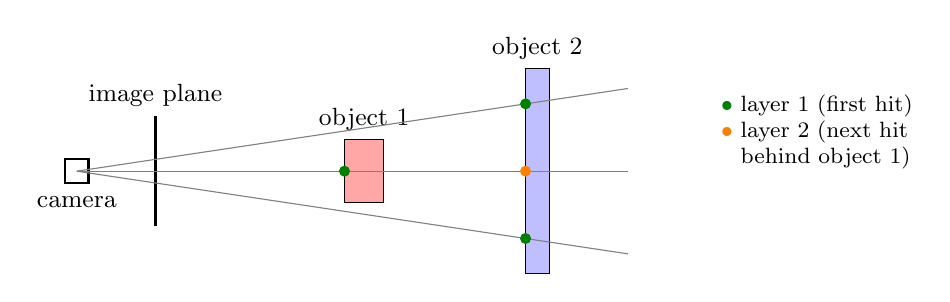
\begin{tikzpicture}[font=\small]
\draw[thick] (-0.15,-0.15) rectangle (0.15,0.15); \node[below] at (0,-0.2) {camera};
\draw[thick] (1,-0.7) -- (1,0.7); \node[above] at (1,0.7) {image plane};
\draw[fill=red!35] (3.4,-0.4) rectangle (3.9,0.4); \node[above] at (3.65,0.4) {object 1};
\draw[fill=blue!25] (5.7,-1.3) rectangle (6.0,1.3); \node[above] at (5.85,1.3) {object 2};
\foreach \s in {0.15,0,-0.15}{\draw[gray] (0,0) -- (7,7*\s);}
\fill[green!50!black] (5.7,0.855) circle (2pt);
\fill[green!50!black] (3.4,0) circle (2pt); \fill[orange] (5.7,0) circle (2pt);
\fill[green!50!black] (5.7,-0.855) circle (2pt);
\node[align=left,font=\footnotesize] at (9.4,0.5) {\textcolor{green!50!black}{$\bullet$} layer 1 (first hit)\\\textcolor{orange}{$\bullet$} layer 2 (next hit\\ \hphantom{$\bullet$} behind object 1)};
\end{tikzpicture}
\caption{Three pixel rays. The upper and lower rays hit only object 2 (layer 1 only); the middle ray hits object 1 first and object 2 second, so its pixel stores two (depth, colour) entries.}
\end{figure}

\begin{intuition}
A depth map keeps only the first hit along each ray; an LDI keeps a \emph{list} of hits. The hidden second layer (what is behind object 1) is what allows rendering from a slightly different viewpoint without holes; but the layer index jumps around from pixel to pixel, so layers are not smooth images.
\end{intuition}

\subsection{Multi-plane Images \slides{slide 70}}
Multi-plane images (MPIs) are discrete volumetric representations with \emph{non-uniform} spatial cells: a stack of fronto-parallel planes at fixed depths, each a (colour, transparency) image. They are extremely efficient to render (each layer is just a plane at fixed depth), but have limited resolution for far-away content; uniform cells may be preferable for object-centric 3D.

\begin{figure}[ht]
\centering
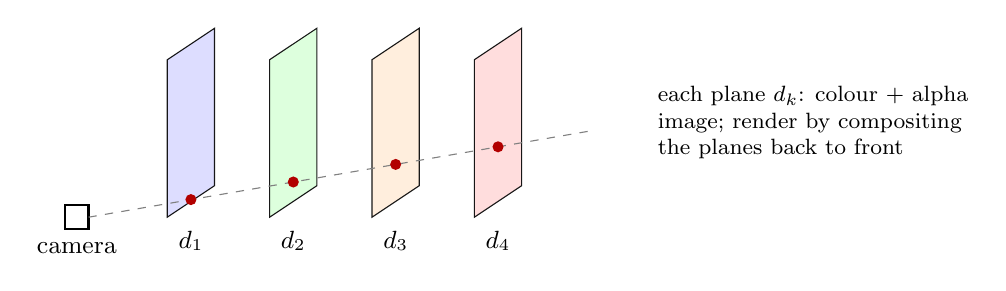
\begin{tikzpicture}[font=\small]
\foreach \k/\c in {0/blue!15,1/green!15,2/orange!15,3/red!15}{
  \draw[fill=\c,opacity=0.9] (\k*1.3,0)--(\k*1.3+0.6,0.4)--(\k*1.3+0.6,2.4)--(\k*1.3,2.0)--cycle;
  \node[below] at (\k*1.3+0.3,-0.05) {$d_{\the\numexpr\k+1\relax}$};
}
\draw[thick] (-1.3,-0.15) rectangle (-1.0,0.15); \node[below] at (-1.15,-0.2) {camera};
\draw[gray,dashed] (-1.0,0) -- (5.4,1.1);
\foreach \k in {0,1,2,3}{\fill[red!70!black] ({\k*1.3+0.3},{(\k*1.3+1.3)*0.1719}) circle (2pt);}
\node[align=left,font=\footnotesize] at (8.2,1.2) {each plane $d_k$: colour + alpha\\image; render by compositing\\the planes back to front};
\end{tikzpicture}
\caption{A multi-plane image: planes at increasing depth $d_1<\dots<d_4$; a pixel ray crosses all of them and the result is their composite.}
\end{figure}

\begin{intuition}
An MPI is a pile of transparent slides at fixed depths: to draw the scene from a nearby viewpoint, shift and blend the slides. Planes are spaced non-uniformly (dense near, sparse far), which is why distant content gets little resolution.
\end{intuition}

\subsection{CAD Models and CSG Trees \slides{slide 71}}
CAD models and CSG (constructive solid geometry) trees are \emph{compositions of primitive volumes or surfaces}. They are popular across design applications but challenging for learning.

\begin{figure}[ht]
\centering
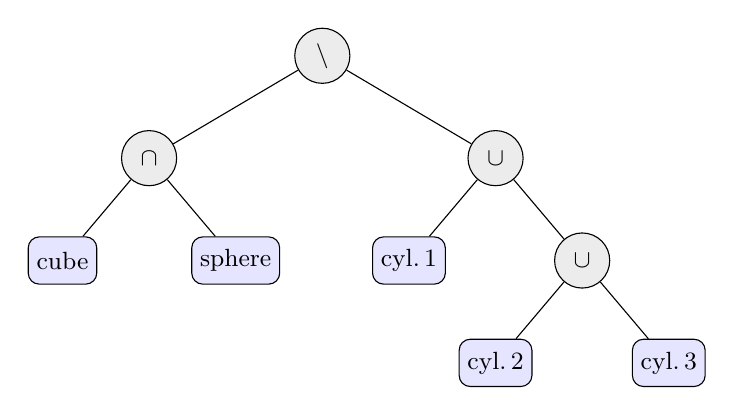
\begin{tikzpicture}[font=\small,
 op/.style={circle,draw,fill=gray!15,minimum size=7mm,inner sep=0pt},
 pr/.style={draw,rounded corners,fill=blue!10,minimum height=6mm,inner sep=3pt}]
\node[op] (r) at (0,0) {$\setminus$};
\node[op] (l) at (-2.2,-1.3) {$\cap$};
\node[op] (rr) at (2.2,-1.3) {$\cup$};
\node[pr] (c) at (-3.3,-2.6) {cube};
\node[pr] (s) at (-1.1,-2.6) {sphere};
\node[pr] (y1) at (1.1,-2.6) {cyl.\,1};
\node[op] (u) at (3.3,-2.6) {$\cup$};
\node[pr] (y2) at (2.2,-3.9) {cyl.\,2};
\node[pr] (y3) at (4.4,-3.9) {cyl.\,3};
\draw (r)--(l) (r)--(rr) (l)--(c) (l)--(s) (rr)--(y1) (rr)--(u) (u)--(y2) (u)--(y3);
\end{tikzpicture}
\caption{A CSG tree: leaves are primitives, inner nodes are Boolean operations (as on slide 71: $(\text{cube}\cap\text{sphere})\setminus(\text{cyl.}_1\cup(\text{cyl.}_2\cup\text{cyl.}_3))$).}
\end{figure}

\begin{example}[A CSG tree is a nested $\min/\max$]
If each primitive has an implicit function ($f_{\text{cube}},f_{\text{sph}},f_{c1},f_{c2},f_{c3}$), the tree of the figure is the field
\[
f=\max\Big(\max(f_{\text{cube}},f_{\text{sph}}),\;-\min\big(f_{c1},\min(f_{c2},f_{c3})\big)\Big),
\]
by the Boolean rules of slide 52.
\end{example}

\begin{intuition}
A CSG model is a \emph{program}: a recipe of primitives and Boolean steps. It is compact, editable and exact, but the structure (which tree, how deep) is discrete and combinatorial, so it is hard to predict with a neural network by gradient descent.
\end{intuition}

% =====================================================================
\section{Summary \slides{slides 72--74}}\label{sec:summary}
% =====================================================================

The summary slide (72) repeats the zoo of slide 4: mesh, point cloud, CAD model, voxels, implicit surface $\{\vx\mid f(\vx)=0\}$, parametric surface $f(\vu)=\vx\in\R^3$, CSG tree, and many more. Slides 73--74 are ``Questions?'' and Acknowledgments: the slides are adapted from \emph{Learning for 3D Vision}, CMU 16-825, Prof.\ Shubham Tulsiani.

\subsection*{Comparison table}
\newcommand{\Y}{\cellcolor{green!25}}
\newcommand{\Pm}{\cellcolor{yellow!30}}
\newcommand{\N}{\cellcolor{red!22}}
\begin{center}
\small
\renewcommand{\arraystretch}{1.3}
\setlength{\tabcolsep}{3pt}\begin{tabular}{L{2.3cm}L{2.3cm}L{2.3cm}L{2.5cm}L{2.3cm}L{2.3cm}}
\toprule
 & \textbf{Get surface points} & \textbf{Inside / outside} & \textbf{Change topology continuously} & \textbf{Render directly} & \textbf{Memory scales with}\\
\midrule
Point cloud & \Y given & \N no surface & \Y any point set & \Pm splats & points ($N$)\\
Triangle mesh & \Y sample triangles & \Pm count ray crossings & \N same wiring only & \Y rasterizer & vertices, faces\\
Parametric & \Y evaluate $f$ & \N search over $\vu$ & \N same topology only & \N via a mesh & parameters of $f$\\
Voxels & \Pm marching cubes & \Y look up cell & \Pm with probabilities & \Pm blocky & $n^3$\\
Implicit / SDF & \Pm marching cubes & \Y sign of $f$ & \Y any topology & \Pm ray marching & grid $n^3$ or network\\
\bottomrule
\end{tabular}
\end{center}
{\noindent\footnotesize \colorbox{green!25}{\strut easy}\quad\colorbox{yellow!30}{\strut possible with effort}\quad\colorbox{red!22}{\strut hard / limited}. Ratings are our reading of slides 22--62 and the table of slide 66, not a table from the slides.}

\begin{figure}[ht]
\centering
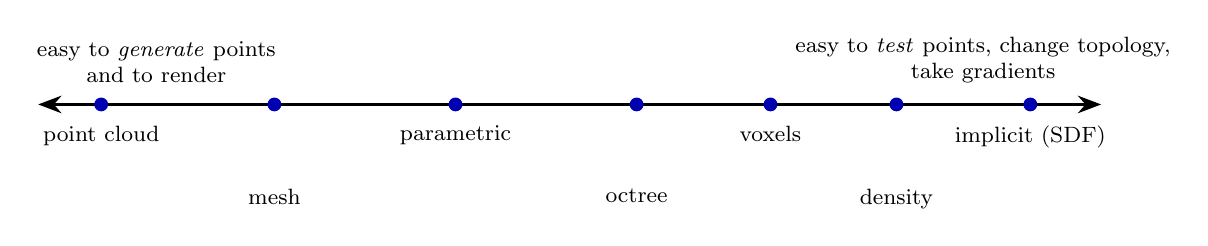
\begin{tikzpicture}[font=\small,>=Stealth]
\draw[<->,very thick] (0,0)--(13.5,0);
\node[above,align=center,font=\footnotesize] at (1.5,0.15) {easy to \emph{generate} points\\and to render};
\node[above,align=center,font=\footnotesize] at (12,0.15) {easy to \emph{test} points, change topology,\\take gradients};
\foreach \x/\t/\y in {0.8/point cloud/-0.6,3.0/mesh/-1.4,5.3/parametric/-0.6,7.6/octree/-1.4,9.3/voxels/-0.6,10.9/density/-1.4,12.6/implicit (SDF)/-0.6}{
  \fill[blue!70!black] (\x,0) circle (2.5pt); \node[below] at (\x,\y+0.45) {\footnotesize\t};
}
\end{tikzpicture}
\caption{A qualitative map of the ``generate vs.\ test'' spectrum (our summary of slides 41, 48, 62 and 66; positions are indicative only).}
\end{figure}

\subsection*{Key take-aways}
\begin{itemize}
\item \textbf{There is no universal 3D representation.} Points and depth maps come from sensors; meshes are for rendering and graphics; implicit fields are for inside/outside tests, topology changes and learning; the right choice depends on the task.
\item \textbf{Parametric generates, implicit tests.} $f(\vu)=\vx$ makes sampling trivial and queries hard; $\{f(\vx)=0\}$ makes queries trivial (sign of $f$, $\nabla f$ for normals, $\min/\max$ for Booleans) and sampling hard.
\item \textbf{Meshes split geometry from connectivity.} $V$ is continuous and optimizable; $F$ is discrete, so predicting arbitrary connectivity or changing topology is hard; check winding order, and remember $F\approx2V$ for closed genus-0 meshes.
\item \textbf{Grids are simple but pay for empty space.} A $n^3$ voxel grid (or SDF grid) handles any topology and suits convolutions, but only $\sim n^2$ cells touch the surface; octrees and continuous fields (networks, Gaussians) fight this cost.
\item \textbf{SDFs are the well-behaved implicit fields.} $\norm{\nabla f}=1$ makes $|f|$ the true distance, enabling safe ray-marching steps and TSDF fusion, and marching cubes converts any such field back into a mesh.
\end{itemize}

% % =====================================================================
% \appendix
% \section{Appendix: Harmonic Functions and the Winding Number \slides{slide 75, backup slide}}\label{app:winding}
% % =====================================================================
% \emph{Supplementary: this slide appears in the file \textbf{after} the Questions and Acknowledgments slides (it is a backup slide), so it is kept out of the main flow.}

% Slide 75 presents the winding number as an alternative implicit function:
% \begin{definition}[Winding number]
% $w(\vx)$ is the signed solid angle of $\Surf$ seen from $\vx$, divided by $4\pi$. On the slide: $w=1$ inside, $w=0$ outside, and the surface sits at $w=\tfrac12$; $w$ is harmonic \emph{away from} the surface; it is robust (holes and noise give fractional values); and it is defined even for an oriented point cloud, which is why reconstruction uses it (slide credits: Barill et al.\ 2018, Gillespie et al.\ 2024, Chen et al.\ 2024).
% \end{definition}

% For a closed surface with outward normals the standard integral form (not written on the slide) is $w(\vx)=\frac1{4\pi}\int_{\Surf}\frac{(\vy-\vx)\cdot\vn(\vy)}{\norm{\vy-\vx}^3}\,dA(\vy)$.

% \begin{figure}[ht]
% \centering
% \begin{tikzpicture}
% \begin{axis}[width=0.75\linewidth,height=5cm,xlabel={position along a line through the unit disk (2D analogue)},ylabel={$w$},xmin=-2,xmax=2,ymin=-0.1,ymax=1.15,ytick={0,0.5,1},grid=both]
% \addplot[thick,blue,const plot] coordinates {(-2,0)(-1,0)(-1,1)(1,1)(1,0)(2,0)};
% \addplot[only marks,mark=*,red] coordinates {(-1,0.5)(1,0.5)};
% \end{axis}
% \end{tikzpicture}
% \caption{2D analogue: $w$ is the angle subtended by the curve divided by $2\pi$. It is $1$ inside, $0$ outside, and exactly $\tfrac12$ on the curve (red dots), where the curve fills half of the viewing directions.}
% \end{figure}

% \begin{intuition}
% Stand at $\vx$ and ask ``what fraction of my full view sphere is covered by the surface, counting front-side coverage positively?'': inside a closed shape you see it all around you (fraction $1$), outside it is cancelled out (front and back cancel, fraction $0$), and standing \emph{on} the surface you are covered on one half (fraction $\tfrac12$). If the surface has a small hole or noise, a point just inside sees slightly less than everything, giving a value like $0.95$ rather than a hard failure. That graceful behaviour makes $w$ useful for turning oriented point clouds into implicit surfaces.
% \end{intuition}

\end{document}